\chapter{架起彩虹桥,我们友谊比天高——把张量当做旋量}

正如我们所预期的,世界张量是旋量的特殊情况,即张量代数是通过复合指标的方式嵌入(embed)在旋量代数中的。在一开始,我们使用正常的描述流形$\mathcal{M}$的办法,即使用世界矢量和世界张量。度规作为一个描述$\mathcal{M}$的几何的特殊张量被引入,随后我们可以使用类光标架定义旋量的概念。同时,为了保证这个旋量的概念在整个时空中都是自洽的,我们需要给流形引入拓扑上的需求。随后旋量可以用复杂的时空几何描述其意义。但实际上我们可能要问,自然是否真的是如此复杂的。



实际上,这种复杂性很大程度上来源于一开始我们就使用了张量方法,如果我们将自旋矢量比世界矢量看做更基本的量,即某些比时空本身的结构更加先验的东西,实际上这些复杂的结构是可以被\textbf{推导}出来的。如果我们直接从旋量出发,那么符号上的模糊性就自然消失了。实际上,我们直接从旋量出发,所得到的时空会自动满足有时间和空间定向,并且有自旋结构,甚至时空的维数和符号都是旋量形式的“结果”。


\section{作为旋量的世界张量}

我们定义世界张量的指标集为
\begin{equation*}
	\mathcal{K} =\{\boldsymbol{a} ,\boldsymbol{b} ,\cdots ,\boldsymbol{z} ,\boldsymbol{a}_{0} ,\cdots \} ,
\end{equation*}
其中每一个指标都是旋量指标$\mathcal{L} ,\mathcal{L} '$的复合指标:
\begin{equation*}
	\boldsymbol{a} =\boldsymbol{AA} ',\boldsymbol{b} =\boldsymbol{BB} ',\cdots \boldsymbol{z} =\boldsymbol{ZZ} ',\cdots .
\end{equation*}
例如我们考虑
\begin{equation*}
	\psi ^{\boldsymbol{AA} '}{}{_{\boldsymbol{BB} '}}^{\boldsymbol{Q}} =\psi ^{\boldsymbol{a}}{}{_{\boldsymbol{BB} '}}^{\boldsymbol{Q}} =\psi ^{\boldsymbol{a}}{}{_{\boldsymbol{b}}}^{\boldsymbol{Q}} =\cdots 
\end{equation*}
注意,旋量指标的运算法则可能隐藏在复合指标中:
\begin{equation*}
	\psi ^{\boldsymbol{AA} '}{}{_{\boldsymbol{BB} '}}^{\boldsymbol{B}} =\psi ^{\boldsymbol{a}}{}{_{\boldsymbol{b}}}^{\boldsymbol{B}} =-\psi ^{\boldsymbol{aB}}{}_{\boldsymbol{b}} .
\end{equation*}
这意味着我们有$\mathfrak{S}^{\boldsymbol{a}} =\mathfrak{S}^{\boldsymbol{AA} '} ,\mathfrak{S}^{\boldsymbol{b}} =\mathfrak{S}^{\boldsymbol{BB} '} \cdots $,这种旋量的特殊之处就在于他们的复共轭在原先的空间中。我们称这样构造出来的张量为\textbf{复世界张量}(complex world-tensor)。可以看出这种旋量的复共轭就是
\begin{equation*}
	\overline{\chi ^{\boldsymbol{a} \cdots \boldsymbol{d}}{}_{\boldsymbol{p} \cdots \boldsymbol{r}}} =\overline{\chi ^{\boldsymbol{AA} '\cdots \boldsymbol{DD} '}{}_{\boldsymbol{PP} '\cdots \boldsymbol{RR} '}} =\overline{\chi }^{\boldsymbol{AA} '\cdots \boldsymbol{DD} '}{}_{\boldsymbol{PP} '\cdots \boldsymbol{RR} '} =\overline{\chi }^{\boldsymbol{a} \cdots \boldsymbol{d}}{}_{\boldsymbol{p} \cdots \boldsymbol{r}} .
\end{equation*}
如果在复共轭操作下不变,那么我们称这样的张量为\textbf{实世界张量}(real world-tensors),即
\begin{equation*}
	\chi ^{\boldsymbol{a} \cdots \boldsymbol{d}}{}_{\boldsymbol{p} \cdots \boldsymbol{r}} =\overline{\chi }^{\boldsymbol{a} \cdots \boldsymbol{d}}{}_{\boldsymbol{p} \cdots \boldsymbol{r}} .
\end{equation*}
我们将只包含实世界张量的$\mathfrak{S} ,\mathfrak{S}^{\boldsymbol{a}} ,\cdots $的子集标记为$\mathfrak{T} ,\mathfrak{T}^{\boldsymbol{a}} ,\cdots $。



我们定义特殊的世界张量(度规张量)为:
\begin{equation}
	g_{\boldsymbol{ab}} =\epsilon _{\boldsymbol{AB}} \epsilon _{\boldsymbol{A} '\boldsymbol{B} '} ,
	\label{eq:4.1}
\end{equation}
那么我们可以看出几个性质:
\begin{equation*}
	g_{\boldsymbol{ab}} =g_{\boldsymbol{ba}} ,g^{\boldsymbol{ab}} =g^{\boldsymbol{ba}} ,g_{\boldsymbol{ab}} g^{\boldsymbol{bc}} =g{_{\boldsymbol{a}}}^{\boldsymbol{c}} ,g_{\boldsymbol{ab}} g^{\boldsymbol{ab}} =4.
\end{equation*}
同时可以证明我们也可以用度规升降指标:
\begin{equation*}
	\chi ^{\mathcal{C}}{}_{\boldsymbol{a}} =\chi ^{\mathcal{C}}{}_{\boldsymbol{b}} g{_{\boldsymbol{a}}}^{\boldsymbol{b}} ,\chi ^{\mathcal{C}\boldsymbol{a}} =\chi ^{\mathcal{C}\boldsymbol{a}} g{_{\boldsymbol{b}}}^{\boldsymbol{a}} ,
\end{equation*}
这意味着$g{_{\boldsymbol{a}}}^{\boldsymbol{b}}$可以被看成克罗内克$\delta $,以及
\begin{equation*}
	\chi ^{\mathcal{C}\boldsymbol{a}} =\chi ^{\mathcal{C}}{}_{\boldsymbol{b}} g^{\boldsymbol{ab}} ,\chi ^{\mathcal{C}}{}_{\boldsymbol{a}} =\chi ^{\mathcal{C}\boldsymbol{b}} g_{\boldsymbol{ab}} .
\end{equation*}
\subsection{自旋标架}

下面我们来看我们上面定义的“世界矢量”是如何与我们日常在相对论理论中使用的张量是同构的。



之前我们已经引入了自旋标架$o^{\boldsymbol{A}} ,\iota ^{\boldsymbol{A}}$,并且采用标准归一化:
\begin{equation*}
	o_{\boldsymbol{A}} \iota ^{\boldsymbol{A}} =1.
\end{equation*}
我们定义世界矢量的\textbf{类光标架}(null tetrad)为
\begin{equation*}
	\begin{aligned}
		l^{\boldsymbol{a}} & =o^{\boldsymbol{A}} o^{\boldsymbol{A} '} , & n^{\boldsymbol{a}} & =\iota ^{\boldsymbol{A}} \iota ^{\boldsymbol{A} '} ,\\
		m^{\boldsymbol{a}} & =o^{\boldsymbol{A}} \iota ^{\boldsymbol{A} '} , & \overline{m}^{\boldsymbol{a}} & =\iota ^{\boldsymbol{A}} o^{\boldsymbol{A} '} .
	\end{aligned}
\end{equation*}
我们可以发现这些都是类光矢量,因为
\begin{equation*}
	l^{\boldsymbol{a}} l_{\boldsymbol{a}} =n^{\boldsymbol{a}} n_{\boldsymbol{a}} =m^{\boldsymbol{a}} m_{\boldsymbol{a}} =\overline{m}^{\boldsymbol{a}}\overline{m}_{\boldsymbol{a}} =0,
\end{equation*}
例如
\begin{equation*}
	m^{\boldsymbol{a}} m_{\boldsymbol{a}} =(o^{\boldsymbol{A}} \iota ^{\boldsymbol{A} '} )(o_{\boldsymbol{A}} \iota _{\boldsymbol{A} '} )=0.
\end{equation*}
同时,
\begin{equation*}
	l^{\boldsymbol{a}} n_{\boldsymbol{a}} =-1,m^{\boldsymbol{a}}\overline{m}_{\boldsymbol{a}} =-1,
\end{equation*}
以及
\begin{equation*}
	l^{\boldsymbol{a}} m_{\boldsymbol{a}} =l^{\boldsymbol{a}}\overline{m}_{\boldsymbol{a}} =n^{\boldsymbol{a}} m_{\boldsymbol{a}} =n^{\boldsymbol{a}}\overline{m}_{\boldsymbol{a}} =0,
\end{equation*}
同时$l^{\boldsymbol{a}} ,n^{\boldsymbol{a}}$都是实的,$m^{\boldsymbol{a}}$和$\overline{m}^{\boldsymbol{a}}$互为复共轭。根据$\epsilon {_{\boldsymbol{A}}}^{\boldsymbol{B}} =o_{\boldsymbol{A}} \iota ^{\boldsymbol{B}} -\iota _{\boldsymbol{A}} o^{\boldsymbol{B}}$我们可以看出
\begin{equation*}
	g{_{\boldsymbol{a}}}^{\boldsymbol{b}} =n_{\boldsymbol{a}} l^{\boldsymbol{a}} +l_{\boldsymbol{a}} n^{\boldsymbol{b}} -\overline{m}_{\boldsymbol{a}} m^{\boldsymbol{b}} -m_{\boldsymbol{a}}\overline{m}^{\boldsymbol{b}} ,
\end{equation*}
这意味着,四个世界矢量构成了一个$\mathfrak{S}^{\boldsymbol{a}}$的基,其对偶基分别为$n_{\boldsymbol{a}} ,l_{\boldsymbol{a}} ,-\overline{m}_{\boldsymbol{a}} ,-m_{\boldsymbol{a}}$。



如果要给出$\mathfrak{T}$上的$\mathfrak{T}^{\boldsymbol{a}}$的基,我们需要实世界矢量,这意味着需要将$m^{\boldsymbol{a}}$和$\overline{m}^{\boldsymbol{a}}$分成实部和虚部。我们可以选取
\begin{equation}
	\begin{aligned}
		& t^{\boldsymbol{a}} =\frac{1}{\sqrt{2}} (l^{\boldsymbol{a}} +n^{\boldsymbol{a}} )=\frac{1}{\sqrt{2}} (o^{\boldsymbol{A}} o^{\boldsymbol{A} '} +\iota ^{\boldsymbol{A}} \iota ^{\boldsymbol{A} '} )\\
		& x^{\boldsymbol{a}} =\frac{1}{\sqrt{2}} (m^{\boldsymbol{a}} +\overline{m}^{\boldsymbol{a}} )=\frac{1}{\sqrt{2}} (o^{\boldsymbol{A}} \iota ^{\boldsymbol{A} '} +\iota ^{\boldsymbol{A}} o^{\boldsymbol{A} '} )\\
		& y^{\boldsymbol{a}} =\frac{1}{\sqrt{2}} (m^{\boldsymbol{a}} -\overline{m}^{\boldsymbol{a}} )=\frac{\mathrm{i}}{\sqrt{2}} (o^{\boldsymbol{A}} \iota ^{\boldsymbol{A} '} -\iota ^{\boldsymbol{A}} o^{\boldsymbol{A} '} )\\
		& z^{\boldsymbol{a}} =\frac{1}{\sqrt{2}} (l^{\boldsymbol{a}} -n^{\boldsymbol{a}} )=\frac{1}{\sqrt{2}} (o^{\boldsymbol{A}} o^{\boldsymbol{A} '} -\iota ^{\boldsymbol{A}} \iota ^{\boldsymbol{A} '} ),
	\end{aligned}
	\label{eq:4.2}
\end{equation}
其逆关系为
\begin{equation*}
	\begin{aligned}
		l^{\boldsymbol{a}} & =\frac{1}{\sqrt{2}} (t^{\boldsymbol{a}} +z^{\boldsymbol{a}} )=o^{\boldsymbol{A}} o^{\boldsymbol{A} '}\\
		n^{\boldsymbol{a}} & =\frac{1}{\sqrt{2}} (t^{\boldsymbol{a}} -z^{\boldsymbol{a}} )=\iota ^{\boldsymbol{A}} \iota ^{\boldsymbol{A} '}\\
		m^{\boldsymbol{a}} & =\frac{1}{\sqrt{2}} (x^{\boldsymbol{a}} -\mathrm{i} y^{\boldsymbol{a}} )=o^{\boldsymbol{A}} \iota ^{\boldsymbol{A} '}\\
		\overline{m}^{\boldsymbol{a}} & =\frac{1}{\sqrt{2}} (x^{\boldsymbol{a}} +\mathrm{i} y^{\boldsymbol{a}} )=\iota ^{\boldsymbol{A}} o^{\boldsymbol{A} '} .
	\end{aligned}
\end{equation*}
我们可以看到四个向量之间是相互正交的,
\begin{equation*}
	t^{\boldsymbol{a}} x_{\boldsymbol{a}} =t^{\boldsymbol{a}} y_{\boldsymbol{a}} =t^{\boldsymbol{a}} z_{\boldsymbol{a}} =x^{\boldsymbol{a}} y_{\boldsymbol{a}} =y^{\boldsymbol{a}} z_{\boldsymbol{a}} =z^{\boldsymbol{a}} x_{\boldsymbol{a}} =0,
\end{equation*}
并且满足归一化关系:
\begin{equation*}
	t^{\boldsymbol{a}} t_{\boldsymbol{a}} =1,x^{\boldsymbol{a}} x_{\boldsymbol{a}} =y^{\boldsymbol{a}} y_{\boldsymbol{a}} =z^{\boldsymbol{a}} z_{\boldsymbol{a}} =-1.
\end{equation*}
同时,我们发现可以将度规写成:
\begin{equation*}
	g{_{\boldsymbol{a}}}^{\boldsymbol{b}} =t_{\boldsymbol{a}} t^{\boldsymbol{b}} -x_{\boldsymbol{a}} x^{\boldsymbol{b}} -y_{\boldsymbol{a}} y^{\boldsymbol{b}} -z_{\boldsymbol{a}} z^{\boldsymbol{b}} .
\end{equation*}
这意味着$t^{\boldsymbol{a}} ,x^{\boldsymbol{a}} ,y^{\boldsymbol{a}} ,z^{\boldsymbol{a}}$确实构成了一个$\mathfrak{T}^{\boldsymbol{a}}$的基底,即闵氏标架 (Minkowski tetrad),其对偶基为$t_{\boldsymbol{a}} ,-x_{\boldsymbol{a}} ,-y_{\boldsymbol{a}} ,-z_{\boldsymbol{a}}$。那么我们可以记这个基为:
\begin{equation}
	g{_{0}}^{\boldsymbol{a}} =t^{\boldsymbol{a}} ,\ \ g{_{1}}^{\boldsymbol{a}} =x^{\boldsymbol{a}} ,\ \ g{_{2}}^{\boldsymbol{a}} =y^{\boldsymbol{a}} ,\ \ g{_{3}}^{\boldsymbol{a}} =z^{\boldsymbol{a}} ,
	\label{eq:4.3}
\end{equation}
以及其对偶基:
\begin{equation*}
	g{_{\boldsymbol{a}}}^{0} =t_{\boldsymbol{a}} ,\ \ g{_{\boldsymbol{a}}}^{1} =-x_{\boldsymbol{a}} ,\ \ g{_{\boldsymbol{a}}}^{2} =-y_{\boldsymbol{a}} ,\ \ g{_{\boldsymbol{a}}}^{3} =-z_{\boldsymbol{a}} .
\end{equation*}
那么度规再这个基底下的分量就为:
\begin{equation*}
	g_{ab} =g_{\boldsymbol{ab}} g{_{a}}^{\boldsymbol{a}} g{_{b}}^{\boldsymbol{b}} =\begin{pmatrix}
		1 &  &  & \\
		& -1 &  & \\
		&  & -1 & \\
		&  &  & -1
	\end{pmatrix} =g^{ab} ,g{_{a}}^{b} =\begin{pmatrix}
		1 &  &  & \\
		& 1 &  & \\
		&  & 1 & \\
		&  &  & 1
	\end{pmatrix} .
\end{equation*}
下面我们尝试\textbf{给出}时间和空间的可定向性。注意到如果我们切换自旋标架$o^{\boldsymbol{A}} ,\iota ^{\boldsymbol{A}}$,那么响应的变换是与单位变换连通的自旋变换,这意味着对应的四标架\ref{eq:4.2}也是通过限制性洛伦兹变换与彼此相连的——即$\mathfrak{T}^{\boldsymbol{a}}$中的方向性是\textbf{内在}的,并不依赖于自旋标架$o^{\boldsymbol{A}} ,\iota ^{\boldsymbol{A}}$的选择。



考虑$K^{\boldsymbol{a}} \in \mathfrak{T}^{\boldsymbol{a}}$,那么我们可以将这个矢量在基底下展开:
\begin{equation}
	K^{\boldsymbol{a}} =K^{a} g{_{a}}^{\boldsymbol{a}} =K^{0} t^{\boldsymbol{a}} +K^{1} x^{\boldsymbol{a}} +K^{2} y^{\boldsymbol{a}} +K^{3} z^{\boldsymbol{a}} ,
	\label{eq:4.4}
\end{equation}
其中
\begin{equation*}
	K^{0} =K^{\boldsymbol{a}} t_{\boldsymbol{a}} ,K^{1} =-K^{\boldsymbol{a}} x_{\boldsymbol{a}} ,K^{2} =-K^{\boldsymbol{a}} y_{\boldsymbol{a}} ,K^{3} =-K^{\boldsymbol{a}} z_{\boldsymbol{a}} .
\end{equation*}
现在考虑在旋量基下的展开:
\begin{equation}
	\begin{aligned}
		K^{\boldsymbol{a}} & =K^{AA'} \epsilon {_{A}}^{\boldsymbol{A}} \epsilon {_{A'}}^{\boldsymbol{A} '}\\
		& =K^{00'} o^{\boldsymbol{A}} o^{\boldsymbol{A} '} +K^{01'} o^{\boldsymbol{A}} l^{\boldsymbol{A} '} +K^{10'} l^{\boldsymbol{A}} o^{\boldsymbol{A} '} +K^{11'} l^{A} l^{A}\\
		& =K^{00'} l^{\boldsymbol{a}} +K^{11'} n^{\boldsymbol{a}} +K^{01'} m^{\boldsymbol{a}} +K^{10'}\overline{m}^{\boldsymbol{a}} .
	\end{aligned}
	\label{eq:4.5}
\end{equation}
对比\ref{eq:4.4}\ref{eq:4.5}\ref{eq:4.2},我们可以发现在矢量基和旋量基下展开系数之间的关系:
\begin{equation*}
	\frac{1}{\sqrt{2}}\begin{pmatrix}
		K^{0} +K^{3} & K^{1} +\mathrm{i} K^{2}\\
		K^{1} -\mathrm{i} K^{2} & K^{0} -K^{3}
	\end{pmatrix} =\begin{pmatrix}
		K^{00'} & K^{01'}\\
		K^{10'} & K^{11'}
	\end{pmatrix} .
\end{equation*}
我们知道洛伦兹群作用在$\mathfrak{T}^{\boldsymbol{a}}$上的效果是将任何一个指向未来的类光矢量变换到另一个,这意味着如果$K^{\boldsymbol{a}}$是指向未来的,那么他是某些旋量和其共轭的乘积:
\begin{equation*}
	K^{\boldsymbol{a}} =\kappa ^{\boldsymbol{A}}\overline{\kappa }^{\boldsymbol{A} '} .
\end{equation*}
这意味着如果我们令
\begin{equation*}
	\xi =\kappa ^{0} ,\eta =\kappa ^{1} ,
\end{equation*}
那么我们知道
\begin{equation*}
	K^{00'} =\xi \overline{\xi } ,K^{01'} =\xi \overline{\eta } ,K^{10'} =\eta \overline{\xi } ,K^{11'} =\eta \overline{\eta } ,
\end{equation*}
那么我们可以给出
\begin{equation*}
	\frac{1}{\sqrt{2}}\begin{pmatrix}
		T+Z & X+\mathrm{i} Y\\
		X-\mathrm{i} Y & T-Z
	\end{pmatrix} =\begin{pmatrix}
		\xi \overline{\xi } & \xi \overline{\eta }\\
		\eta \overline{\xi } & \eta \overline{\eta }
	\end{pmatrix} =\begin{pmatrix}
		\xi \\
		\eta 
	\end{pmatrix}\begin{pmatrix}
		\overline{\xi } & \overline{\eta }
	\end{pmatrix} ,
\end{equation*}
这里
\begin{equation*}
	T=K^{0} ,X=K^{1} ,Y=K^{2} ,Z=K^{3} .
\end{equation*}
这是第一章的基础,这意味着如果我们从$\mathcal{M}$及其度规$g_{\boldsymbol{ab}}$出发,同时如果$\mathcal{M}$满足允许让我们构建旋量的全局条件,那么度规$g_{\boldsymbol{ab}}$与这里我们通过\ref{eq:4.1}构建的度规是一致的。


\subsection{英费尔德-范德瓦尔登符号}

现在我们考虑,如果选取$\mathfrak{S}^{\boldsymbol{a}}$与$\mathfrak{S}^{\boldsymbol{A}}$中的\textbf{任意}两组基,那么一个张量在这两组基下面的分量之间有什么关系?注意,这里$\mathfrak{S}^{\boldsymbol{a}}$的基的选取并不是直接从$\mathfrak{S}^{\boldsymbol{A}}$中诱导出来的。



考虑实世界矢量$\chi {_{\boldsymbol{a} \cdots \boldsymbol{c}}}^{\boldsymbol{d} \cdots \boldsymbol{f}}$在$\mathfrak{T}^{\boldsymbol{a}}$的基$g{_{a}}^{\boldsymbol{a}}$下展开的系数与$\chi {_{\boldsymbol{AA} '\cdots \boldsymbol{CC} '}}^{\boldsymbol{DD} '\cdots \boldsymbol{FF} '}$在$\epsilon {_{A}}^{\boldsymbol{A}}$下的展开系数,它们之间实际上由所谓的英费尔德-范德瓦尔登符号(Infeld-van der Waerden symbols)连接:
\begin{equation*}
	\begin{aligned}
		g{_{a}}^{AA'} & \equiv g{_{a}}^{\boldsymbol{a}} \epsilon {_{\boldsymbol{A}}}^{A} \epsilon {_{\boldsymbol{A} '}}^{A'} ,\\
		g{_{AA'}}^{a} & \equiv \epsilon {_{A}}^{\boldsymbol{A}} \epsilon {_{A'}}^{\boldsymbol{A} '} g{_{\boldsymbol{a}}}^{a} .
	\end{aligned}
\end{equation*}
注意,这里具体指标并没有缩并,只有抽象指标有缩并\footnote{根据我们的记号,缩并仅发生在下列情况中:
	\begin{itemize}
		\item 种类完全一致的指标,例如$B{_{a}}^{a} ,B{_{\boldsymbol{a}}}^{\boldsymbol{a}} ,E{_{A}}^{A} ,E{_{\boldsymbol{A}}}^{\boldsymbol{A}} ,D{_{\mathcal{C}}}^{\mathcal{C}}$
		\item 抽象复合指标和显示指标,例如$F_{\boldsymbol{a}} G^{\boldsymbol{A}} ,F_{\boldsymbol{a}} G^{\boldsymbol{A}} H^{\boldsymbol{A} '}$
\end{itemize}}。例如我们有
\begin{equation*}
	\begin{aligned}
		\chi {_{a\cdots c}}^{d\cdots f} & =\chi {_{AA'\cdots CC'}}^{DD'\cdots FF'} g{_{a}}^{AA'} \cdots g{_{c}}^{CC'} g{_{DD'}}^{d} \cdots g{_{FF'}}^{f} ,\\
		\chi {_{AA'\cdots CC'}}^{DD'\cdots FF'} & =\chi {_{a\cdots c}}^{d\cdots f} g{_{AA'}}^{a} \cdots g{_{CC'}}^{c} g{_{d}}^{DD'} \cdots g{_{f}}^{FF'} .
	\end{aligned}
\end{equation*}
由于$g{_{a}}^{\boldsymbol{a}} \in \mathfrak{T}^{\boldsymbol{a}}$是实的,我们知道
\begin{equation*}
	\overline{g{_{a}}^{AB'}} =g{_{a}}^{\boldsymbol{a}} \epsilon {_{\boldsymbol{A} '}}^{A'} \epsilon {_{\boldsymbol{A}}}^{B} =g{_{a}}^{BA'} ,
\end{equation*}
这意味着矩阵$g{_{0}}^{AB'} ,\cdots g{_{3}}^{AB'}$是厄米的。那么,如果$\chi {_{\boldsymbol{a} \cdots \boldsymbol{c}}}^{\boldsymbol{d} \cdots \boldsymbol{f}}$是实的世界张量,那么其旋量分量一定是厄米的:
\begin{equation}
	\overline{\chi {_{AP'\cdots CR'}}^{DS'\cdots FU'}} =\chi {_{PA'\cdots RC'}}^{SD'\cdots UF'} .
	\label{eq:4.6}
\end{equation}
需要注意的是,方程$\overline{\chi {_{\cdots }}^{\cdots }} =\chi {_{\cdots }}^{\cdots }$通常是无意义的,因为两个模$\mathfrak{S}^{\boldsymbol{A} '} ,\mathfrak{S}^{\boldsymbol{A}}$中的元素没有可比性。但对于$\{( p,r) ,( p,r)\}$类的旋量这是有意义的,因为这样方程就变成了
\begin{equation*}
	\overline{\chi }{_{C'D\cdots }}^{A'B\cdots } =\chi {_{C'D\cdots }}^{A'B\cdots } ,
\end{equation*}
而这与条件\ref{eq:4.6}不同,我们称\ref{eq:4.6}是\textbf{厄米}的,而上式是\textbf{实}的。



我们也可以考虑度规的分量,根据\ref{eq:4.1},我们知道
\begin{equation}
	g_{ab} =\epsilon _{AB} \epsilon _{A'B'} g{_{a}}^{AA'} g{_{b}}^{BB'} ,
	\label{eq:4.7}
\end{equation}
或者等价的我们有
\begin{equation*}
	g_{ab} g{_{AA'}}^{a} g{_{BB'}}^{b} =\epsilon _{AB} \epsilon _{A'B'} .
\end{equation*}
如果我们将\ref{eq:4.7}的$ab$指标对称化,我们有:
\begin{equation*}
	\epsilon ^{CD} (g_{ab} +g_{ba} )=(\epsilon _{A'B'} g{_{a}}^{AA'} g{_{b}}^{BB'} +\epsilon _{A'B'} g{_{b}}^{AA'} g{_{a}}^{BB'} )\epsilon _{AB} \epsilon ^{CD}
\end{equation*}
利用恒等式

\begin{equation*}
	\epsilon {_{A}}^{C} \epsilon {_{B}}^{D} -\epsilon {_{B}}^{C} \epsilon {_{A}}^{D} =\epsilon _{AB} \epsilon ^{CD} ,
\end{equation*}再升降指标,并重命名哑标指标,利用$g_{ab} =g_{ba}$,我们给出
\begin{equation*}
	\begin{aligned}
		-\epsilon {_{B}}^{A} (g_{ab} +g_{ba} ) & =2(g{_{a}}^{A}{}_{B'} g_{b}{}{_{B}}^{B'} +g{_{b}}^{A}{}_{B'} g_{a}{}{_{B}}^{B'} ),
	\end{aligned}
\end{equation*}
即
\begin{equation*}
	-\epsilon {_{B}}^{A} g_{ab} =g{_{a}}^{A}{}_{B'} g_{b}{}{_{B}}^{B'} +g{_{b}}^{A}{}_{B'} g_{a}{}{_{B}}^{B'} .
\end{equation*}
这个等式就是著名的Clifford代数的定义式,即我们可以将上式写成
\begin{equation}
	G_{a} G_{b}^{\dagger } +G_{b} G_{a}^{\dagger } =-g_{ab}\boldsymbol{I}_{2} ,
	\label{eq:4.8}
\end{equation}
其中如果我们令
\begin{equation*}
	\gamma _{a} \equiv \frac{1}{\sqrt{2}}\begin{pmatrix}
		0 & G_{a}\\
		G_{a}^{\dagger } & 0
	\end{pmatrix} ,
\end{equation*}
那么我们可以将\ref{eq:4.8}写成
\begin{equation*}
	\gamma _{a} \gamma _{b} +\gamma _{b} \gamma _{a} =-2g_{ab}\boldsymbol{I}_{4} .
\end{equation*}
如果我们用标准的闵氏标架$t^{\boldsymbol{a}} ,x^{\boldsymbol{a}} ,y^{\boldsymbol{a}} ,z^{\boldsymbol{a}}$,那么可以计算出
\begin{equation*}
	\begin{aligned}
		g{_{0}}^{AB'} & =\frac{1}{\sqrt{2}}\begin{pmatrix}
			1 & 0\\
			0 & 1
		\end{pmatrix} =g{_{AB'}}^{0} =\frac{1}{\sqrt{2}} \sigma ^{0} , & g{_{1}}^{AB'} & =\frac{1}{\sqrt{2}}\begin{pmatrix}
			0 & 1\\
			1 & 0
		\end{pmatrix} =g{_{AB'}}^{1} =\frac{1}{\sqrt{2}} \sigma ^{1} ,\\
		g{_{2}}^{AB'} & =\frac{1}{\sqrt{2}}\begin{pmatrix}
			0 & \mathrm{i}\\
			-\mathrm{i} & 0
		\end{pmatrix} =-g{_{AB'}}^{2} =\frac{1}{\sqrt{2}} \sigma ^{2} , & g{_{3}}^{AB'} & =\frac{1}{\sqrt{2}}\begin{pmatrix}
			1 & 0\\
			0 & -1
		\end{pmatrix} =g{_{AB'}}^{3} =\frac{1}{\sqrt{2}} \sigma ^{3} .
	\end{aligned}
\end{equation*}
这正好是泡利矩阵。有时候我们也会使用类光标架,但这个标架不是实的,而是复的,即使用标架$g{_{0}}^{\boldsymbol{a}} =l^{a} ,g{_{1}}^{\boldsymbol{a}} =n^{a} ,g{_{2}}^{\boldsymbol{a}} =m^{a} ,g{_{3}}^{\boldsymbol{a}} =\overline{m}^{a}$,这里我们有
\begin{equation*}
	\begin{aligned}
		g{_{0}}^{AB'} & =\begin{pmatrix}
			1 & 0\\
			0 & 0
		\end{pmatrix} =g{_{AB'}}^{0} , & g{_{1}}^{AB'} & =\begin{pmatrix}
			0 & 0\\
			0 & 1
		\end{pmatrix} =g{_{AB'}}^{1} ,\\
		g{_{2}}^{AB'} & =\begin{pmatrix}
			0 & 1\\
			0 & 0
		\end{pmatrix} =g{_{AB'}}^{2} , & g{_{3}}^{AB'} & =\begin{pmatrix}
			0 & 0\\
			1 & 0
		\end{pmatrix} =g{_{AB'}}^{3} .
	\end{aligned}
\end{equation*}
由于$g{_{a}}^{\boldsymbol{a}}$不是实的,这里$g{_{a}}^{\boldsymbol{AB} '}$自然也不是厄米的。


\section{光旗和类光矢量*}

之前我们通过张量用时空几何的方法给出了自旋矢量几何解释,但从张量代数出发我们能给出一样的结果,而且更加简单和自然。


\subsection{光旗}

考虑$P\in \mathcal{M}$一点的旋量,这里$\mathfrak{S} \cong \mathbb{C}$,那么$\mathfrak{S}^{\boldsymbol{A}}$是一个二维向量空间。考虑$\kappa ^{\boldsymbol{A}} \in \mathfrak{S}^{\boldsymbol{A}}$,我们可以构造一个世界矢量:
\begin{equation}
	K^{\boldsymbol{a}} =\kappa ^{\boldsymbol{A}}\overline{\kappa }^{\boldsymbol{A} '} ,
	\label{eq:4.9}
\end{equation}
这个世界矢量明显是实的,而且他还是类光的,因为
\begin{equation*}
	K^{\boldsymbol{a}} K_{\boldsymbol{a}} =\left| \kappa _{\boldsymbol{A}} \kappa ^{\boldsymbol{A}}\right| ^{2} =0.
\end{equation*}
事实上,每一个\textbf{实的}类光的世界矢量要么是\ref{eq:4.9}的形式,要么是
\begin{equation*}
	K^{\boldsymbol{a}} =-\kappa ^{\boldsymbol{A}}\overline{\kappa }^{\boldsymbol{A} '}
\end{equation*}
的形式。同时,任何一个复的世界矢量$\chi ^{\boldsymbol{a}}$是类光的,即
\begin{equation}
	\chi ^{\boldsymbol{a}} \chi _{\boldsymbol{a}} =0
	\label{eq:4.10}
\end{equation}
等价于它可以被写成
\begin{equation}
	\chi ^{\boldsymbol{a}} =\kappa ^{\boldsymbol{A}} \xi ^{\boldsymbol{A} '} .
	\label{eq:4.11}
\end{equation}
为了看出\ref{eq:4.10}能给出\ref{eq:4.11},只需要将其写成旋量形式,即
\begin{equation*}
	\epsilon _{\boldsymbol{AB}} \epsilon _{\boldsymbol{A} '\boldsymbol{B} '} \chi ^{\boldsymbol{AA} '} \chi ^{\boldsymbol{BB} '} =0,
\end{equation*}
而如果将上式写成分量形式,正好为$2\chi ^{00'} \chi ^{11'} -2\chi ^{01'} \chi ^{10'} =2\det \chi ^{AA'}$,其为零意味着$\chi ^{AA'}$的秩小于$2$,因此可以被拆成两个旋量的外乘,即\ref{eq:4.11}。

如果$\chi ^{\boldsymbol{a}}$是实的,我们给出$\kappa ^{\boldsymbol{A}} \xi ^{\boldsymbol{A} '} =\overline{\xi }^{\boldsymbol{A}}\overline{\kappa }^{\boldsymbol{A} '}$,将这个方程两边对$\overline{\xi }_{\boldsymbol{A}}$缩并,我们知道
\begin{equation*}
	(\overline{\xi }_{\boldsymbol{A}} \kappa ^{\boldsymbol{A}} )\xi ^{\boldsymbol{A} '} =0,
\end{equation*}
即$\overline{\xi }^{\boldsymbol{A}}$必须是$\kappa ^{\boldsymbol{A}}$的标量倍,即$\chi ^{\boldsymbol{a}} =q\kappa ^{\boldsymbol{A}}\overline{\kappa }^{\boldsymbol{A} '}$,其中$q$是实数。如果$q >0$,将因子$\sqrt{q}$吸收进$\kappa $的定义,这就给出了\ref{eq:4.9}的形式,如果$q< 0$,将$\sqrt{-q}$吸收进定义,就给出了第二种情况。这两种情况分别对应了光锥指向未来的部分和指向过去的部分。当我们考虑$\mathcal{M}$上的旋量场的时候,时间定向性就这样被给出了。



注意到方程\ref{eq:4.9}告诉我们任意一个非零的自旋矢量定义了一个唯一的指向未来的类光矢量,我们称其为\textbf{旗杆}(flagpole)。但我们发现,不同的自旋矢量能给出相同的旗杆,即$K^{\boldsymbol{a}}$有自由度
\begin{equation}
	\kappa ^{\boldsymbol{A}} \mapsto \mathrm{e}^{\mathrm{i} \theta } \kappa ^{\boldsymbol{A}} .
	\label{eq:4.12}
\end{equation}
为了给出$\kappa ^{\boldsymbol{A}}$真正的张量版本,我们考虑定义$P^{\boldsymbol{ab}}$为:
\begin{equation}
	P^{\boldsymbol{ab}} =\kappa ^{\boldsymbol{A}} \kappa ^{\boldsymbol{B}} \epsilon ^{\boldsymbol{A} '\boldsymbol{B} '} +\epsilon ^{\boldsymbol{AB}}\overline{\kappa }^{\boldsymbol{A} '}\overline{\kappa }^{\boldsymbol{B} '} .
	\label{eq:4.13}
\end{equation}
这个$P^{\boldsymbol{ab}}$就是单个旋量$\kappa ^{\boldsymbol{A}}$的张量实现。我们可以看出这个量是实的,并且是反对称的:
\begin{equation*}
	P^{\boldsymbol{ab}} =\overline{P}^{\boldsymbol{ba}} =-P^{\boldsymbol{ba}} .
\end{equation*}
实际上,如果我们将$\kappa ^{\boldsymbol{A}}$当成一个基向量的话,选取另一个基向量为$\tau ^{\boldsymbol{A}}$,以及归一化
\begin{equation*}
	\kappa _{\boldsymbol{A}} \tau ^{\boldsymbol{A}} =1,
\end{equation*}
那么而我们有
\begin{equation*}
	\epsilon ^{\boldsymbol{AB}} =\kappa ^{\boldsymbol{A}} \tau ^{\boldsymbol{B}} -\tau ^{\boldsymbol{A}} \kappa ^{\boldsymbol{B}} ,
\end{equation*}
将其带入定义,我们可以给出
\begin{equation*}
	P^{\boldsymbol{ab}} =K^{\boldsymbol{a}} L^{\boldsymbol{b}} -L^{\boldsymbol{a}} K^{\boldsymbol{b}} ,
\end{equation*}
其中
\begin{equation*}
	L^{\boldsymbol{a}} \equiv \kappa ^{\boldsymbol{A}}\overline{\tau }^{\boldsymbol{A} '} +\tau ^{\boldsymbol{A}}\overline{\kappa }^{\boldsymbol{A} '} .
\end{equation*}
我们可以发现$L^{\boldsymbol{a}}$是实的,类空的并且长度为$-\sqrt{2}$,以及与$K^{\boldsymbol{a}}$正交:
\begin{equation*}
	\overline{L^{\boldsymbol{a}}} =L^{\boldsymbol{a}} ,L^{\boldsymbol{a}} L_{\boldsymbol{a}} =-2,K^{\boldsymbol{a}} L_{\boldsymbol{a}} =0.
\end{equation*}
实际上,即使这样,我们发现在变换
\begin{equation*}
	\tau ^{\boldsymbol{A}}\rightarrow \tau ^{\boldsymbol{A}} +\alpha \kappa ^{\boldsymbol{A}}
\end{equation*}
下,
\begin{equation*}
	L^{\boldsymbol{a}}\rightarrow L^{\boldsymbol{a}} +( \alpha +\overline{\alpha }) K^{\boldsymbol{a}} ,
\end{equation*}
而$P\boldsymbol{^{ab}}$在这个变换下不变,这意味着$L^{\boldsymbol{a}}$有一个“半平面”的冗余自由度。这个半平面穿过闵氏向量空间$\mathfrak{T}^{\boldsymbol{a}}$的圆点,并且与光锥正交,我们将其称作$\kappa ^{\boldsymbol{A}}$的\textbf{光旗面}(flag plane)。



事实上,\ref{eq:4.12}给出的相位变化对应了旗面绕旗杆旋转$2\theta $。在变换\ref{eq:4.12}下,为了保证内积不变,我们需要令$\tau ^{\boldsymbol{A}} \mapsto \mathrm{e}^{-\mathrm{i} \theta } \tau ^{\boldsymbol{A}}$。那么在这个变换下:
\begin{equation*}
	\begin{aligned}
		L^{\boldsymbol{a}} =\kappa ^{\boldsymbol{A}}\overline{\tau }^{\boldsymbol{A} '} +\tau ^{\boldsymbol{A}}\overline{\kappa }^{\boldsymbol{A} '} & \mapsto (\mathrm{e}^{\mathrm{i} \theta } \kappa ^{\boldsymbol{A}} )(\mathrm{e}^{\mathrm{i} \theta }\overline{\tau }^{\boldsymbol{A} '} )+(\mathrm{e}^{-\mathrm{i} \theta } \tau ^{\boldsymbol{A}} )(\mathrm{e}^{-\mathrm{i} \theta }\overline{\kappa }^{\boldsymbol{A} '} )\\
		& =(\cos 2\theta +\mathrm{i}\sin 2\theta )\kappa ^{\boldsymbol{A}}\overline{\tau }^{\boldsymbol{A} '} +(\cos 2\theta -\mathrm{i}\sin 2\theta )\tau ^{\boldsymbol{A}}\overline{\kappa }^{\boldsymbol{A} '}\\
		& =\cos 2\theta (\kappa ^{\boldsymbol{A}}\overline{\tau }^{\boldsymbol{A} '} +\tau ^{\boldsymbol{A}}\overline{\kappa }^{\boldsymbol{A} '} )+\sin 2\theta (\mathrm{i} \kappa ^{\boldsymbol{A}}\overline{\tau }^{\boldsymbol{A} '} -\mathrm{i} \tau ^{\boldsymbol{A}}\overline{\kappa }^{\boldsymbol{A} '} ),
	\end{aligned}
\end{equation*}
如果我们定义
\begin{equation*}
	M^{\boldsymbol{a}} =\mathrm{i} \kappa ^{\boldsymbol{A}}\overline{\tau }^{\boldsymbol{A} '} -\mathrm{i} \tau ^{\boldsymbol{A}}\overline{\kappa }^{\boldsymbol{A} '} ,
\end{equation*}
那么我们有
\begin{equation*}
	L^{\boldsymbol{a}} \mapsto L^{\boldsymbol{a}}\cos 2\theta +M^{\boldsymbol{a}}\sin 2\theta ,
\end{equation*}
即$L^{\boldsymbol{a}}$在$(L^{\boldsymbol{a}} ,M^{\boldsymbol{a}} )$平面上旋转了$2\theta $。如果我们定义“右手性”(right-handed)为旗面随着转动$\mathrm{e}^{\mathrm{i} \theta } \kappa ^{\boldsymbol{A}}$的转角$\theta $增加的方向,那么$\mathcal{M}$的空间定向性就自然出现了。同时,注意到$\theta =\pi $时旗面转动了$2\pi $,回到原先的位置但$\kappa ^{\boldsymbol{A}} \mapsto -\kappa ^{\boldsymbol{A}}$,这意味着$\kappa ^{\boldsymbol{A}}$是一个旋量对象。那么通过我们的代数方法,$\mathcal{M}$上的旋量结构自然浮现了。


\subsection{复类光矢量}

现在我们考虑一般的复类光矢量$\chi ^{\boldsymbol{a}} =\kappa ^{\boldsymbol{A}} \xi ^{\boldsymbol{A} '}$。这个分解在变换
\begin{equation*}
	\kappa ^{\boldsymbol{A}} \mapsto \lambda \kappa ^{\boldsymbol{A}} ,\xi ^{\boldsymbol{A} '} \mapsto \lambda ^{-1} \xi ^{\boldsymbol{A} '}
\end{equation*}
下是不变的,而且在这个意义下也是唯一定义的。例如考虑有另外一组自旋矢量$\mu ^{\boldsymbol{A}} \nu ^{\boldsymbol{A} '}$满足$\kappa ^{\boldsymbol{A}} \xi ^{\boldsymbol{A} '} =\mu ^{\boldsymbol{A}} \nu ^{\boldsymbol{A} '}$,那么对$\mu _{\boldsymbol{A}}$缩并我们给出$\mu _{\boldsymbol{A}} \kappa ^{\boldsymbol{A}} =0$,即$\kappa ^{\boldsymbol{A}}$与$\mu ^{\boldsymbol{A}}$成正比,同理$\xi ^{\boldsymbol{A} '}$与$\nu ^{\boldsymbol{A} '}$成正比。这意味着一个复的类光矢量定义了一对实的类光矢量,分别由$\kappa ^{\boldsymbol{A}} ,\xi ^{\boldsymbol{A} '}$的旗杆给出,当$\chi ^{\boldsymbol{a}}$为实矢量的时候,两个类光方向重合。



我们可以给出一些简单结论。当两个类光矢量$\chi ^{\boldsymbol{a}} ,\psi ^{\boldsymbol{a}}$是正交的时候,即$\chi _{\boldsymbol{a}} \psi ^{\boldsymbol{a}} =0$,我们知道它们两个一定能被写成
\begin{equation*}
	\chi ^{\boldsymbol{a}} =\kappa ^{\boldsymbol{A}} \xi ^{\boldsymbol{A} '} ,\psi ^{\boldsymbol{a}} =\kappa ^{\boldsymbol{A}} \eta ^{\boldsymbol{A} '}
\end{equation*}
或
\begin{equation*}
	\chi ^{\boldsymbol{a}} =\kappa ^{\boldsymbol{A}} \xi ^{\boldsymbol{A} '} ,\psi ^{\boldsymbol{a}} =\tau ^{\boldsymbol{A}} \xi ^{\boldsymbol{A} '} .
\end{equation*}
如果三个类光矢量两两正交,那么他们一定是线性相关的,因为他们总可以被写成
\begin{equation*}
	\chi ^{\boldsymbol{a}} =\kappa ^{\boldsymbol{A}} \xi ^{\boldsymbol{A} '} ,\psi ^{\boldsymbol{a}} =\kappa ^{\boldsymbol{A}} \eta ^{\boldsymbol{A} '} ,\phi ^{\boldsymbol{a}} =\kappa ^{\boldsymbol{A}} \zeta ^{\boldsymbol{A} '}
\end{equation*}
或其共轭的形式。


\subsection{厄米类光矢量}

最后考虑这种复类光矢量,满足:
\begin{equation*}
	\gamma ^{\boldsymbol{a}}\overline{\gamma }_{\boldsymbol{a}} =0.
\end{equation*}
我们可以将这个矢量写成
\begin{equation*}
	\gamma ^{\boldsymbol{a}} =\mathrm{e}^{\mathrm{i} \theta } (U^{\boldsymbol{a}} +\mathrm{i} V^{\boldsymbol{a}} ),\theta \in \mathbb{R} ,
\end{equation*}
其中$U^{\boldsymbol{a}} ,V^{\boldsymbol{a}}$都是实矢量。将上式带入定义,我们给出
\begin{equation*}
	U_{\boldsymbol{a}} U^{\boldsymbol{a}} +V_{\boldsymbol{a}} V^{\boldsymbol{a}} =0.
\end{equation*}
这意味着要么$U,V$都是类光的,要么一个类光一个类空。但我们总能调节$\theta $,让两个都是类空的并且是指向未来的,除非$U,V$都为零或者他们本就正相关。对于后者,我们可以直接写出
\begin{equation*}
	\gamma ^{\boldsymbol{a}} =\mathrm{e}^{\mathrm{i} \theta } U^{\boldsymbol{a}} ,
\end{equation*}
其中$U^{\boldsymbol{a}}$是实的,类光的并且指向未来的。如果我们将其拆成旋量表示,对于以上两种情况我们有
\begin{equation*}
	\gamma ^{\boldsymbol{a}} =\begin{cases}
		\mathrm{e}^{\mathrm{i} \theta } (\alpha ^{\boldsymbol{A}}\overline{\alpha }^{\boldsymbol{A} '} +\mathrm{i} \beta ^{\boldsymbol{A}}\overline{\beta }^{\boldsymbol{A} '} ) & \alpha _{\boldsymbol{A}} \beta ^{\boldsymbol{A}} \neq 0\\
		\mathrm{e}^{\mathrm{i} \theta } \alpha ^{\boldsymbol{A}}\overline{\alpha }^{\boldsymbol{A} '} & \alpha _{\boldsymbol{A}} =\lambda \beta _{\boldsymbol{A}}
	\end{cases} .
\end{equation*}

\section{对称化操作}

我们来考虑张(旋)量运算中最重要的对称化/反对称化操作,虽然后者在二维的旋量空间中几乎是没有用处的。我们需要用到的性质仅仅只有可加性以及完全自反性。


\subsection{对称化与反对称化}

我们使用指标上的圆(方)括号表示指标的(反)对称化,即:
\begin{equation*}
	\chi _{\mathcal{P} (\boldsymbol{ab} )\mathcal{Q}} =\frac{1}{2!} (\chi _{\mathcal{P}\boldsymbol{ab}\mathcal{Q}} +\chi _{\mathcal{P}\boldsymbol{ba}\mathcal{Q}} ),
\end{equation*}
以及
\begin{equation*}
	\chi _{\mathcal{P}[\boldsymbol{ab}]\mathcal{Q}} =\frac{1}{2!} (\chi _{\mathcal{P}\boldsymbol{ab}\mathcal{Q}} -\chi _{\mathcal{P}\boldsymbol{ba}\mathcal{Q}} ).
\end{equation*}
有时候我们会需要有些指标不做对称化或反对称化,但又无法随意交换指标的位置,因此采用竖线将不参与对称操作的指标隔离:
\begin{equation*}
	\phi {_{\boldsymbol{a} (\boldsymbol{b}}}^{\boldsymbol{c}}{}_{|\boldsymbol{l} |\boldsymbol{n} )} =\frac{1}{2!} (\phi {_{\boldsymbol{ab}}}^{\boldsymbol{c}}{}_{\boldsymbol{ln}} +\phi {_{\boldsymbol{an}}}^{\boldsymbol{c}}{}_{\boldsymbol{lb}} ),
\end{equation*}
甚至
\begin{equation*}
	\theta ^{(\boldsymbol{a}| \boldsymbol{b}[\boldsymbol{cl}]| \boldsymbol{n})} =\frac{1}{2} (\theta ^{\boldsymbol{a}| \boldsymbol{b}[\boldsymbol{cl}]| \boldsymbol{n}} +\theta ^{\boldsymbol{n}| \boldsymbol{b}[\boldsymbol{cl}]| \boldsymbol{a}} )=\frac{1}{4} (\theta ^{\boldsymbol{abcln}} -\theta ^{\boldsymbol{ablcn}} +\theta ^{\boldsymbol{nbcla}} -\theta ^{\boldsymbol{nblca}} ).
\end{equation*}
我们可以给出这两种操作的一些性质。



首先,对于同样的操作的复合,内层可以被忽略,例如$\eta _{\boldsymbol{a}((\boldsymbol{ln})\boldsymbol{m})} =\eta _{\boldsymbol{a}(\boldsymbol{lnm})}$,或$\xi _{\boldsymbol{a}[\boldsymbol{b}[\boldsymbol{cl}]]} =\xi _{\boldsymbol{a}[\boldsymbol{bcl}]}$。如果是不同操作的复合,那么结果为零:
\begin{equation*}
	\chi _{\mathcal{P}[\boldsymbol{a} \cdots (\boldsymbol{c} \cdots \boldsymbol{l}) \cdots \boldsymbol{n}]\mathcal{Q}} =\chi _{\mathcal{P}(\boldsymbol{a} \cdots [\boldsymbol{c} \cdots \boldsymbol{l}] \cdots \boldsymbol{n})\mathcal{Q}} =0.
\end{equation*}
但需要注意,当指标有交叉而不是完全包含的时候,这样的表达式是不允许的,因为对称化操作彼此之间并不交换,例如像$\psi _{\boldsymbol{a}(\boldsymbol{bc}[\boldsymbol{l})\boldsymbol{ns}]}$这样的表达式就不被允许,但$\psi _{(\boldsymbol{ab})\boldsymbol{c}[\boldsymbol{lns}]}$这样的表达式是没有歧义的。但对于不同的上下标,这样的操作就是允许的,因为上下标是独立的,例如:
\begin{equation*}
	\theta ^{[\boldsymbol{a}}{}{_{(\boldsymbol{l}}}^{\boldsymbol{b}]}{}{_{\boldsymbol{n})}}^{\boldsymbol{g}} =\frac{1}{4} (\theta ^{\boldsymbol{a}}{}{_{\boldsymbol{l}}}^{\boldsymbol{b}}{}{_{\boldsymbol{n}}}^{\boldsymbol{g}} -\theta ^{\boldsymbol{b}}{}{_{\boldsymbol{l}}}^{\boldsymbol{a}}{}{_{\boldsymbol{n}}}^{\boldsymbol{g}} +\theta ^{\boldsymbol{a}}{}{_{\boldsymbol{n}}}^{\boldsymbol{b}}{}{_{\boldsymbol{l}}}^{\boldsymbol{g}} -\theta ^{\boldsymbol{b}}{}{_{\boldsymbol{n}}}^{\boldsymbol{a}}{}{_{\boldsymbol{l}}}^{\boldsymbol{g}} ).
\end{equation*}
如果是相同操作有交叉指标,那么操作可以复合,即如果
\begin{equation*}
	\chi _{\cdots \boldsymbol{a} \cdots \boldsymbol{b} \cdots \boldsymbol{c} \cdots } =\chi _{\cdots (\boldsymbol{a} \cdots \boldsymbol{b}) \cdots \boldsymbol{c} \cdots } =\chi _{\cdots \boldsymbol{a} \cdots (\boldsymbol{b} \cdots \boldsymbol{c}) \cdots } ,
\end{equation*}
那么
\begin{equation*}
	\chi _{\cdots \boldsymbol{a} \cdots \boldsymbol{b} \cdots \boldsymbol{c} \cdots } =\chi _{\cdots (\boldsymbol{a} \cdots \boldsymbol{b} \cdots \boldsymbol{c}) \cdots } ,
\end{equation*}
这对反对称操作也适用。



由于对于$X^{\boldsymbol{a}} \in \mathfrak{S}^{\boldsymbol{a}}$,张量$X^{\boldsymbol{a}} X^{\boldsymbol{b}} \cdots X^{\boldsymbol{c}}$都是对称的,我们给出这样的定理:

\begin{them}[label={them:zero symmetric spinor}]{对称张量为零的条件}
	如果一个对称张量为零,即
	\begin{equation*}
		\phi _{\mathcal{A}(\boldsymbol{ab} \cdots \boldsymbol{c})} =0,
	\end{equation*}
	那么当且仅当对于所有$X^{\boldsymbol{a}} \in \mathfrak{S}^{\boldsymbol{a}}$,都有
	\begin{equation*}
		\phi _{\mathcal{A}\boldsymbol{ab} \cdots \boldsymbol{c}} X^{\boldsymbol{a}} X^{\boldsymbol{b}} \cdots X^{\boldsymbol{c}} =0.
	\end{equation*}
\end{them}

这意味着我们可以定义一个函数:
\begin{equation*}
	\phi _{\mathcal{A}}( X) \equiv \phi _{\mathcal{A}\boldsymbol{ab} \cdots \boldsymbol{c}} X^{\boldsymbol{a}} X^{\boldsymbol{b}} \cdots X^{\boldsymbol{c}} ,
\end{equation*}
这个函数定义了一个对称张量$\phi _{\mathcal{A}(\boldsymbol{ab} \cdots \boldsymbol{c})}$。


\subsection{应用到旋量和张量上}

旋量的特殊性在于它是二维的,并且基底是反对称的,这导致了如果出现三个及以上\textbf{反对称}的旋量指标,那么它们一定为零,即对于任何$\theta _{\mathcal{A}\boldsymbol{PQR}}$或$\theta _{\mathcal{A}\boldsymbol{P} '\boldsymbol{Q} '\boldsymbol{R} '}$,我们一定有
\begin{equation*}
	\theta _{\mathcal{A}[\boldsymbol{PQR}]} =\theta _{\mathcal{A}[\boldsymbol{P} '\boldsymbol{Q} '\boldsymbol{R} ']} =0.
\end{equation*}
因为只要我们拿旋量基$\epsilon {_{A}}^{\boldsymbol{A}}$展开,那么我们会发现一定有一个基出现了至少两次,那么这两个基的指标是对称的:
\begin{equation*}
	\theta _{\mathcal{A} PQR} =\theta _{\mathcal{A}\boldsymbol{PQR}} \epsilon {_{P}}^{\boldsymbol{P}} \epsilon {_{Q}}^{\boldsymbol{Q}} \epsilon {_{R}}^{\boldsymbol{R}} ,
\end{equation*}
对于$P,Q,R\in \{1,2\}$的任何全排列都是零。这个结果告诉我们
\begin{equation*}
	\epsilon _{[\boldsymbol{AB}} \epsilon _{\boldsymbol{C}]\boldsymbol{D}} =0,
\end{equation*}
而这等价于
\begin{equation*}
	\epsilon _{\boldsymbol{AB}} \epsilon _{\boldsymbol{CD}} +\epsilon _{\boldsymbol{BC}} \epsilon _{\boldsymbol{AD}} +\epsilon _{\boldsymbol{CA}} \epsilon _{\boldsymbol{BD}} =0.
\end{equation*}
而这个等式给出了
\begin{equation}
	\phi _{\mathcal{D}\boldsymbol{AB}} =\frac{1}{2} \phi {_{\mathcal{D}\boldsymbol{C}}}^{\boldsymbol{C}} \epsilon _{\boldsymbol{AB}} .
	\label{eq:4.14}
\end{equation}
实际上,这个关系也可以被推广到$n$维。考虑$\mathfrak{S}^{\boldsymbol{a}}$有一个$n$维的基底$\delta _{a}^{\boldsymbol{a}}$,那么我们实际上有
\begin{equation*}
	\chi _{\mathcal{A}[\boldsymbol{a}_{0}\boldsymbol{a}_{1} \cdots \boldsymbol{a}_{n}]} =0.
\end{equation*}
可以类似于二维定义Levi-Civita张量:$\epsilon _{\boldsymbol{a}_{1} \cdots \boldsymbol{a}_{n}}$,实际上我们有:
\begin{equation}
	n!\delta _{\boldsymbol{b}_{1}}^{[\boldsymbol{a}_{1}} \cdots \delta _{\boldsymbol{b}_{1}}^{\boldsymbol{a}_{n}]} =\epsilon ^{\boldsymbol{a}_{1} \cdots \boldsymbol{a}_{n}} \epsilon _{\boldsymbol{b}_{1} \cdots \boldsymbol{b}_{n}} .
	\label{eq:4.15}
\end{equation}
那么对于任何反对称张量$\psi _{\mathcal{A}[\boldsymbol{a}_{1} \cdots \boldsymbol{a}_{n}]}$,我们都可以类似\ref{eq:4.14}“抽出”一个Levi-Civita张量:
\begin{equation*}
	\psi _{\mathcal{A}\boldsymbol{b}_{1} \cdots \boldsymbol{b}_{n}} =\psi _{\mathcal{A}\boldsymbol{a}_{1} \cdots \boldsymbol{a}_{n}} \delta _{\boldsymbol{b}_{1}}^{[\boldsymbol{a}_{1}} \cdots \delta _{\boldsymbol{b}_{1}}^{\boldsymbol{a}_{n}]} =\left(\frac{1}{n!} \psi _{\mathcal{A}\boldsymbol{a}_{1} \cdots \boldsymbol{a}_{n}} \epsilon ^{\boldsymbol{a}_{1} \cdots \boldsymbol{a}_{n}}\right) \epsilon _{\boldsymbol{b}_{1} \cdots \boldsymbol{b}_{n}} .
\end{equation*}
这意味着任意全反对称张量都互相成正比。对于一般情况来说,$\epsilon _{\boldsymbol{a}_{1} \cdots \boldsymbol{a}_{n}}$依赖于基$\delta _{a}^{\boldsymbol{a}}$的选择,但对于旋量,由于内积的存在,我们可以针对自旋标架选出一个特定的$\epsilon _{\boldsymbol{AB}}$,而对于世界张量,由于度规的存在,我们出于特别的考量选择$e^{\boldsymbol{abcd}} \in \mathfrak{T}^{\boldsymbol{abcd}}$,称其为置换张量(alternating tensor):
\begin{equation}
	e_{\boldsymbol{abcd}} \equiv \mathrm{i} \epsilon \boldsymbol{_{AC}} \epsilon \boldsymbol{_{BD}} \epsilon _{\boldsymbol{A'D} '} \epsilon _{\boldsymbol{B} '\boldsymbol{C} '} -\mathrm{i} \epsilon _{\boldsymbol{AD}} \epsilon _{\boldsymbol{BC}} \epsilon \boldsymbol{_{A'C'}} \epsilon \boldsymbol{_{B'D'}} .
	\label{eq:4.16}
\end{equation}
我们可以看到,这是个实张量,同时关于$\boldsymbol{a} ,\boldsymbol{b}$和$\boldsymbol{c} ,\boldsymbol{d}$分别是反对称的,因为
\begin{equation*}
	e_{\boldsymbol{bacd}} =\mathrm{i} \epsilon _{\boldsymbol{BC}} \epsilon _{\boldsymbol{AD}} \epsilon \boldsymbol{_{B'D'}} \epsilon \boldsymbol{_{A'C'}} -\mathrm{i} \epsilon \boldsymbol{_{BD}} \epsilon \boldsymbol{_{AC}} \epsilon _{\boldsymbol{B} '\boldsymbol{C} '} \epsilon _{\boldsymbol{A'D} '} =-e_{\boldsymbol{abcd}} .
\end{equation*}
同时,如果交换指标$\boldsymbol{b} ,\boldsymbol{c}$,我们有:
\begin{equation*}
	\begin{aligned}
		& e_{\boldsymbol{abcd}} +e_{\boldsymbol{acbd}}\\
		= & \mathrm{i}( \epsilon _{\boldsymbol{AC}} \epsilon _{\boldsymbol{BD}} -\epsilon _{\boldsymbol{AB}} \epsilon _{\boldsymbol{CD}}) \epsilon _{\boldsymbol{A} '\boldsymbol{D} '} \epsilon _{\boldsymbol{B} '\boldsymbol{C} '} -\mathrm{i} \epsilon _{\boldsymbol{AD} '} \epsilon _{\boldsymbol{BC}}( \epsilon _{\boldsymbol{A} '\boldsymbol{C} '} \epsilon _{\boldsymbol{B} '\boldsymbol{D} '} -\epsilon _{\boldsymbol{A} '\boldsymbol{B} '} \epsilon _{\boldsymbol{C} '\boldsymbol{D} '})\\
		= & \mathrm{i}( \epsilon _{\boldsymbol{AD}} \epsilon _{\boldsymbol{BC}}) \epsilon _{\boldsymbol{A} '\boldsymbol{D} '} \epsilon _{\boldsymbol{B} '\boldsymbol{C} '} -\mathrm{i} \epsilon _{\boldsymbol{AD}} \epsilon _{\boldsymbol{BC}}( \epsilon _{\boldsymbol{A} '\boldsymbol{D} '} \epsilon _{\boldsymbol{B} '\boldsymbol{C} '}) =0.
	\end{aligned}
\end{equation*}
这意味着
\begin{equation*}
	e_{\boldsymbol{abcd}} =e_{[\boldsymbol{abcd}]} .
\end{equation*}
那么我们知道
\begin{equation}
	e_{\boldsymbol{abcd}} e^{\boldsymbol{abcd}} =-24.
	\label{eq:4.17}
\end{equation}
如果我们使用闵氏标架\ref{eq:4.3}以及旋量标架$\{o^{\boldsymbol{A}} ,\iota ^{\boldsymbol{A}} \}$,我们有
\begin{equation*}
	\begin{aligned}
		e_{0123} = & e_{\boldsymbol{abcd}} t^{\boldsymbol{a}} x^{\boldsymbol{b}} y^{\boldsymbol{c}} z^{\boldsymbol{d}}\\
		= & -\frac{1}{4}( \epsilon \boldsymbol{_{AC}} \epsilon \boldsymbol{_{BD}} \epsilon _{\boldsymbol{A'D} '} \epsilon _{\boldsymbol{B} '\boldsymbol{C} '} -\epsilon _{\boldsymbol{AD}} \epsilon _{\boldsymbol{BC}} \epsilon \boldsymbol{_{A'C'}} \epsilon \boldsymbol{_{B'D'}})\\
		& (o^{\boldsymbol{A}} o^{\boldsymbol{A} '} +\iota ^{\boldsymbol{A}} \iota ^{\boldsymbol{A} '} )(o^{\boldsymbol{B}} \iota ^{\boldsymbol{B} '} +\iota ^{\boldsymbol{B}} o^{\boldsymbol{B} '} )(o^{\boldsymbol{C}} \iota ^{\boldsymbol{C} '} -\iota ^{\boldsymbol{C}} o^{\boldsymbol{C} '} )(o^{\boldsymbol{D}} o^{\boldsymbol{D} '} -\iota ^{\boldsymbol{D}} \iota ^{\boldsymbol{D} '} )\\
		= & -\frac{1}{4} (-1-1-1-1 )=1.
	\end{aligned}
\end{equation*}
用度规$g^{ab} =\operatorname{diag}( 1,-1,-1,-1)$升指标给出$e^{0123} =-1$。这意味着
\begin{equation*}
	e_{\boldsymbol{abcd}} =24g{_{[\boldsymbol{a}}}^{0} g{_{\boldsymbol{b}}}^{1} g{_{\boldsymbol{c}}}^{2} g{_{\boldsymbol{d}]}}^{3} =-24t_{[\boldsymbol{a}} x_{\boldsymbol{b}} y_{\boldsymbol{c}} z_{\boldsymbol{d}]} ,
\end{equation*}
同时有
\begin{equation*}
	e^{\boldsymbol{abcd}} =-24g{_{0}}^{[\boldsymbol{a}} g{_{1}}^{\boldsymbol{b}} g{_{2}}^{\boldsymbol{c}} g{_{3}}^{\boldsymbol{d}]} =-24t^{[\boldsymbol{a}} x^{\boldsymbol{b}} y^{\boldsymbol{c}} z^{\boldsymbol{d}]} .
\end{equation*}
实际上,式\ref{eq:4.17}还可以被写成
\begin{equation*}
	-24=e_{\boldsymbol{abcd}} e_{\boldsymbol{pqrs}} g^{\boldsymbol{ap}} g^{\boldsymbol{bq}} g^{\boldsymbol{cr}} g^{\boldsymbol{ds}} =(e_{0123} )^{2} 24\det (g^{ab} )=-24(e_{0123} )^{2} ,
\end{equation*}
这意味着我们选择$e_{0123}  >0$实际上是选择了一个正规(proper)标架。从式\ref{eq:4.15}我们给出
\begin{equation*}
	e_{\boldsymbol{abcd}} e^{\boldsymbol{pqrs}} =-24g{_{\boldsymbol{a}}}^{[\boldsymbol{p}} g{_{\boldsymbol{b}}}^{\boldsymbol{q}} g{_{\boldsymbol{c}}}^{\boldsymbol{r}} g{_{\boldsymbol{d}}}^{\boldsymbol{s}]} ,
\end{equation*}
对指标缩并,我们给出
\begin{equation*}
	\begin{aligned}
		e_{\boldsymbol{abcd}} e^{\boldsymbol{pqrd}} & =-6g{_{\boldsymbol{a}}}^{[\boldsymbol{p}} g{_{\boldsymbol{b}}}^{\boldsymbol{q}} g{_{\boldsymbol{c}}}^{\boldsymbol{r}} g{_{\boldsymbol{d}}}^{\boldsymbol{s}]}\\
		e_{\boldsymbol{abcd}} e^{\boldsymbol{pqcd}} & =-4g{_{\boldsymbol{a}}}^{[\boldsymbol{p}} g{_{\boldsymbol{b}}}^{\boldsymbol{q}]}\\
		e_{\boldsymbol{abcd}} e^{\boldsymbol{pbcd}} & =-6g{_{\boldsymbol{a}}}^{\boldsymbol{p}} .
	\end{aligned}
\end{equation*}
如果定义
\begin{equation*}
	e{_{\boldsymbol{ab}}}^{\boldsymbol{cd}} =\mathrm{i} \epsilon {_{\boldsymbol{A}}}^{\boldsymbol{C}} \epsilon {_{\boldsymbol{B}}}^{\boldsymbol{D}} \epsilon {_{\boldsymbol{A} '}}^{\boldsymbol{D} '} \epsilon {_{\boldsymbol{B} '}}^{\boldsymbol{C} '} -\mathrm{i} \epsilon {_{\boldsymbol{A}}}^{\boldsymbol{D}} \epsilon {_{\boldsymbol{B}}}^{\boldsymbol{C}} \epsilon {_{\boldsymbol{A} '}}^{\boldsymbol{C} '} \epsilon {_{\boldsymbol{B} '}}^{\boldsymbol{D} '} ,
\end{equation*}
那么有
\begin{equation*}
	e{_{\boldsymbol{ab}}}^{\boldsymbol{cd}} e{_{\boldsymbol{cd}}}^{\boldsymbol{pq}} =-4g{_{\boldsymbol{a}}}^{[\boldsymbol{p}} g{_{\boldsymbol{b}}}^{\boldsymbol{q}]} .
\end{equation*}
同时,对于任意张量$H_{\boldsymbol{cd}}$,我们有:
\begin{equation*}
	e{_{\boldsymbol{ab}}}^{\boldsymbol{cd}} H_{\boldsymbol{cd}} =e{_{\boldsymbol{AA} '\boldsymbol{BB} '}}^{\boldsymbol{CC} '\boldsymbol{DD} '} H_{\boldsymbol{CC} '\boldsymbol{DD} '} =\mathrm{i}( H_{\boldsymbol{AB} '\boldsymbol{A} '\boldsymbol{B}} -H_{\boldsymbol{A} '\boldsymbol{BAB} '}) .
\end{equation*}


如果考虑三个指标的反对称张量,我们考虑令
\begin{equation*}
	\begin{aligned}
		& \tilde{e}_{\boldsymbol{abc}} =e_{\boldsymbol{abcd}} \delta {_{0}}^{\boldsymbol{d}}\\
		= & (\mathrm{i} \epsilon \boldsymbol{_{AC}} \epsilon \boldsymbol{_{BD}} \epsilon _{\boldsymbol{A'D} '} \epsilon _{\boldsymbol{B} '\boldsymbol{C} '} -\mathrm{i} \epsilon _{\boldsymbol{AD}} \epsilon _{\boldsymbol{BC}} \epsilon \boldsymbol{_{A'C'}} \epsilon \boldsymbol{_{B'D'}} )t^{\boldsymbol{d}}\\
		= & \frac{1}{\sqrt{2}} (\mathrm{i} \epsilon \boldsymbol{_{AC}} \epsilon \boldsymbol{_{BD}} \epsilon _{\boldsymbol{A'D} '} \epsilon _{\boldsymbol{B} '\boldsymbol{C} '} -\mathrm{i} \epsilon _{\boldsymbol{AD}} \epsilon _{\boldsymbol{BC}} \epsilon \boldsymbol{_{A'C'}} \epsilon \boldsymbol{_{B'D'}} )(o^{\boldsymbol{D}} o^{\boldsymbol{D} '} +\iota ^{\boldsymbol{D}} l^{\boldsymbol{D} '} )\\
		= & \frac{\mathrm{i}}{\sqrt{2}} (\epsilon \boldsymbol{_{AC}} \epsilon _{\boldsymbol{B} '\boldsymbol{C} '}( o_{\boldsymbol{B}} o_{\boldsymbol{A} '} +\iota _{\boldsymbol{B}} \iota _{\boldsymbol{A} '}) -\epsilon _{\boldsymbol{BC}} \epsilon \boldsymbol{_{A'C'}}( o_{\boldsymbol{A}} o_{\boldsymbol{B} '} +\iota _{\boldsymbol{A}} \iota _{\boldsymbol{B} '}) )
	\end{aligned}
\end{equation*}
这个形式下的反对称性不像四维时那么明显,不过显然$\tilde{e}_{\boldsymbol{abc}} =\tilde{e}_{[\boldsymbol{ab}]\boldsymbol{c}}$,而
\begin{equation*}
	\begin{aligned}
		& \tilde{e}_{\boldsymbol{abc}} +\tilde{e}_{\boldsymbol{acb}}\\
		= & \frac{\mathrm{i}}{\sqrt{2}} (\epsilon \boldsymbol{_{AC}} \epsilon _{\boldsymbol{B} '\boldsymbol{C} '}( o_{\boldsymbol{B}} o_{\boldsymbol{A} '} +\iota _{\boldsymbol{B}} \iota _{\boldsymbol{A} '}) -\epsilon _{\boldsymbol{BC}} \epsilon \boldsymbol{_{A'C'}}( o_{\boldsymbol{A}} o_{\boldsymbol{B} '} +\iota _{\boldsymbol{A}} \iota _{\boldsymbol{B} '}) )\\
		& +\frac{\mathrm{i}}{\sqrt{2}} (\epsilon \boldsymbol{_{A\boldsymbol{B}}} \epsilon _{\boldsymbol{C} '\boldsymbol{B} '}( o_{\boldsymbol{C}} o_{\boldsymbol{A} '} +\iota _{\boldsymbol{C}} \iota _{\boldsymbol{A} '}) -\epsilon _{\boldsymbol{CB}} \epsilon \boldsymbol{_{A'\boldsymbol{B} '}}( o_{\boldsymbol{A}} o_{\boldsymbol{C} '} +\iota _{\boldsymbol{A}} \iota _{\boldsymbol{C} '}) )\\
		= & \frac{\mathrm{i}}{\sqrt{2}}[ \epsilon _{\boldsymbol{B} '\boldsymbol{C} '} \epsilon _{\boldsymbol{BC}}( o_{\boldsymbol{A} '} o_{\boldsymbol{A}} +\iota _{\boldsymbol{A} '} \iota _{\boldsymbol{A}}) -\epsilon _{\boldsymbol{BC}} \epsilon _{\boldsymbol{B} '\boldsymbol{C} '}( o_{\boldsymbol{A} '} o_{\boldsymbol{A}} +\iota _{\boldsymbol{A} '} \iota _{\boldsymbol{A}})] =0
	\end{aligned}
\end{equation*}
这意味着$\tilde{e}_{\boldsymbol{abc}} =\tilde{e}_{\boldsymbol{a}[\boldsymbol{bc}]}$,故$\tilde{e}_{\boldsymbol{abc}} =\tilde{e}_{[\boldsymbol{abc}]}$。因此同样我们有
\begin{equation*}
	\begin{aligned}
		e_{\boldsymbol{abc}} e^{\boldsymbol{pqr}} & =-6g{_{\boldsymbol{a}}}^{[\boldsymbol{p}} g{_{\boldsymbol{b}}}^{\boldsymbol{q}} g{_{\boldsymbol{c}}}^{\boldsymbol{r}]}\\
		e_{\boldsymbol{abc}} e^{\boldsymbol{pqc}} & =-2g{_{\boldsymbol{a}}}^{[\boldsymbol{p}} g{_{\boldsymbol{b}}}^{\boldsymbol{q}]}\\
		e_{\boldsymbol{abc}} e^{\boldsymbol{pbc}} & =-2g{_{\boldsymbol{a}}}^{\boldsymbol{p}}\\
		e_{\boldsymbol{abc}} e^{\boldsymbol{abc}} & =-6.
	\end{aligned}
\end{equation*}

\subsection{对称旋量}

本节我们会证明一个重要结论:每一个旋量都可以用全对称旋量表示。考虑最简单的$\phi _{\boldsymbol{AB}}$作为例子,我们知道
\begin{equation*}
	\begin{aligned}
		\phi _{\boldsymbol{AB}} & =\phi _{(\boldsymbol{AB})} +\phi _{[\boldsymbol{AB}]}\\
		& =\theta _{\boldsymbol{AB}} +\lambda \epsilon _{\boldsymbol{AB}} ,
	\end{aligned}
\end{equation*}
其中$\theta _{\boldsymbol{AB}} \equiv \phi _{(\boldsymbol{AB})}$,且$\lambda =\phi {_{\boldsymbol{C}}}^{\boldsymbol{C}} /2$,即$\phi $和$\lambda $都是对称的。



我们用$\sim $标记这样的等价关系,如果两个旋量的差是$\epsilon $外乘一个类型比原来的旋量更低的类型的旋量,例如
\begin{equation*}
	\phi _{\boldsymbol{AB}} \sim \theta _{\boldsymbol{AB}} +\lambda \epsilon _{\boldsymbol{AB}} \sim \psi _{\boldsymbol{AB}} +\epsilon _{\boldsymbol{AC}} \chi ^{\boldsymbol{C}}{}_{\boldsymbol{B}} \cdots 
\end{equation*}
我们希望证明的是
\begin{equation*}
	\phi _{\mathcal{C}\boldsymbol{AB} \cdots \boldsymbol{F}} \sim \phi _{\mathcal{C}(\boldsymbol{AB} \cdots \boldsymbol{F})} .
\end{equation*}
我们知道
\begin{equation}
	\phi _{\mathcal{C}(\boldsymbol{AB} \cdots \boldsymbol{F})} =\frac{1}{r}( \phi _{\mathcal{C}\boldsymbol{A}(\boldsymbol{BC} \cdots \boldsymbol{F})} +\phi _{\mathcal{C}\boldsymbol{B}(\boldsymbol{AC} \cdots \boldsymbol{F})} +\cdots +\phi _{\mathcal{C}\boldsymbol{F}(\boldsymbol{AB} \cdots \boldsymbol{E})}) ,
	\label{eq:4.18}
\end{equation}
其中$r$是指标数。那么我们知道对于等式右边的任意两项,我们有
\begin{equation*}
	\phi _{\mathcal{C}\boldsymbol{A}(\boldsymbol{BC} \cdots \boldsymbol{F})} -\phi _{\mathcal{C}\boldsymbol{C}(\boldsymbol{AB} \cdots \boldsymbol{F})} =-\epsilon _{\boldsymbol{AC}} \phi {_{\mathcal{C}}}^{\boldsymbol{X}}{}_{(\boldsymbol{BXD} \cdots \boldsymbol{F})} ,
\end{equation*}
那么将\ref{eq:4.18}右边第二项开始全部利用上式用$\phi _{\mathcal{C}\boldsymbol{A( BC} \cdots \boldsymbol{F})}$替换,我们知道
\begin{equation*}
	\phi _{\mathcal{C}(\boldsymbol{AB} \cdots \boldsymbol{F})} \sim \phi _{\mathcal{C}\boldsymbol{A}(\boldsymbol{BC} \cdots \boldsymbol{F})} .
\end{equation*}
重复这个论证,我们给出
\begin{equation*}
	\phi _{\mathcal{C}(\boldsymbol{AB} \cdots \boldsymbol{F})} \sim \phi _{\mathcal{C}\boldsymbol{A}(\boldsymbol{BC} \cdots \boldsymbol{F})} \sim \phi _{\mathcal{C}\boldsymbol{AB}(\boldsymbol{C} \cdots \boldsymbol{F})} \sim \cdots \sim \phi _{\mathcal{C}\boldsymbol{AB} \cdots \boldsymbol{F}} .
\end{equation*}
这意味着我们可以给出这样的定理:

\begin{them}[label={them:syemmtric part of a spinor}]{旋量与其对称部分}
	任意一个旋量$\chi _{\boldsymbol{A} \cdots \boldsymbol{FP} '\cdots \boldsymbol{S} '}$是其对称部分$\chi _{(\boldsymbol{A\cdots F})(\boldsymbol{P} '\cdots \boldsymbol{S} ')}$以及$\epsilon $与更低阶旋量的外乘的和。
\end{them}

例如,对于一个三个指标的旋量,我们有
\begin{equation*}
	\chi _{\boldsymbol{ABC}} =\chi _{(\boldsymbol{ABC})} -\frac{1}{3} \epsilon _{\boldsymbol{AB}} \chi ^{\boldsymbol{D}}{}_{(\boldsymbol{DC})} -\frac{1}{3} \epsilon _{\boldsymbol{AC}} \chi ^{\boldsymbol{D}}{}_{(\boldsymbol{DB})} -\frac{1}{2} \epsilon _{\boldsymbol{BC}} \chi {_{\boldsymbol{A}}}^{\boldsymbol{D}}{}_{\boldsymbol{D}} ,
\end{equation*}
以及
\begin{equation*}
	\theta _{\boldsymbol{ABA} '\boldsymbol{B} '} =\theta _{(\boldsymbol{AB} )(\boldsymbol{A} '\boldsymbol{B} ')} -\frac{1}{2} \epsilon _{\boldsymbol{AB}} \theta ^{\boldsymbol{C}}{}_{\boldsymbol{C}(\boldsymbol{A} '\boldsymbol{B} ')} -\frac{1}{2} \epsilon _{\boldsymbol{A} '\boldsymbol{B} '} \theta {_{(\boldsymbol{AB} )}}\boldsymbol{^{\boldsymbol{C} '}{}}_{\boldsymbol{C}} +\frac{1}{4} \epsilon _{\boldsymbol{AB} '} \epsilon _{\boldsymbol{A} '\boldsymbol{B} '} \theta ^{\boldsymbol{C}}{}{_{\boldsymbol{C}}}^{\boldsymbol{C} '}{}_{\boldsymbol{C} '} .
\end{equation*}
我们给出这样的定理:

\begin{them}[label={requirement of a symmetric spinor}]{对称旋量的要求}
	如果一个旋量$\psi _{\boldsymbol{A} \cdots \boldsymbol{DP} \cdots \boldsymbol{SU} '\cdots \boldsymbol{W} '\boldsymbol{F} '\cdots \boldsymbol{H} '}$是对称的,那么当且仅当$\psi _{\boldsymbol{A} \cdots \boldsymbol{DF} '\cdots \boldsymbol{H} '}^{\boldsymbol{U} '\cdots \boldsymbol{W} '\boldsymbol{P} \cdots \boldsymbol{S}}$在四组指标中都是对称的,即
	\begin{equation*}
		\psi _{\boldsymbol{A} \cdots \boldsymbol{DF} '\cdots \boldsymbol{H} '}^{\boldsymbol{U} '\cdots \boldsymbol{W} '\boldsymbol{P} \cdots \boldsymbol{S}} =\psi _{(\boldsymbol{A \cdots D)}(\boldsymbol{F} '\cdots \boldsymbol{H} ')}^{(\boldsymbol{U} '\cdots \boldsymbol{W} ')(\boldsymbol{P} \cdots \boldsymbol{S})} ,
	\end{equation*}
	并且每组指标之间的缩并都为零,即
	\begin{equation*}
		\psi _{\boldsymbol{P} \cdots \boldsymbol{DF} '\cdots \boldsymbol{H} '}^{\boldsymbol{U} '\cdots \boldsymbol{W} '\boldsymbol{P} \cdots \boldsymbol{S}} =0,\psi _{\boldsymbol{A} \cdots \boldsymbol{DU} '\cdots \boldsymbol{H} '}^{\boldsymbol{U} '\cdots \boldsymbol{W} '\boldsymbol{P} \cdots \boldsymbol{S}} =0.
	\end{equation*}
\end{them}


\subsection{可约性——又见杨图}

对称旋量之所以重要是因为它们在$SL( 2,\mathbb{C})$的作用下是\textbf{不可约}(irreducible)的。



我们考虑群$G$的线性表示,其表示空间记为$\mathfrak{B}$,如果$\mathfrak{B}$可以被表示成直和的形式:
\begin{equation*}
	\mathfrak{B} =\mathfrak{B}_{1} \oplus \mathfrak{B}_{2} ,
\end{equation*}
那么我们称这个表示是可约的,否则是不可约的。如果$\mathfrak{B}$可以被表示成不可约表示子空间的直和,那么这样的表示就被称为\textbf{完全可约}(completely reducible)的。



对于我们考虑的$SL( 2,\mathbb{C})$或$PSL( 2,\mathbb{C})$群,可以证明,这两个群的所有有限维表示都是完全可约的,而对于不可约表示,可以使用作用在对称旋量上的方法实现。我们知道旋量自然构成了一个$SL( 2,\mathbb{C})$的表示空间,即$\xi _{\boldsymbol{A}} \mapsto t{_{\boldsymbol{A}}}^{\boldsymbol{B}} \xi _{\boldsymbol{B}}$,其中$t{_{\boldsymbol{A}}}^{\boldsymbol{B}}$是一个自旋变换($SL( 2,\mathbb{C})$中的元素)。如果$\phi _{\boldsymbol{A} \cdots \boldsymbol{CD} '\cdots \boldsymbol{F} '}$是一个对称旋量,那么它的变换形式自然为
\begin{equation*}
	\phi _{\boldsymbol{A} \cdots \boldsymbol{CD} '\cdots \boldsymbol{F} '} \mapsto t{_{\boldsymbol{A}}}^{\boldsymbol{A}_{0}} \cdots t{_{\boldsymbol{C}}}^{\boldsymbol{C}_{0}}\overline{t}{_{\boldsymbol{D} '}}^{\boldsymbol{D} '_{0}} \cdots \overline{t}{_{\boldsymbol{F} '}}^{\boldsymbol{F} '_{0}} \phi _{\boldsymbol{A}_{0} \cdots \boldsymbol{C}_{0}\boldsymbol{D} '_{0} \cdots \boldsymbol{F} '_{0}} ,
\end{equation*}
即
\begin{equation*}
	\phi _{\mathcal{A}} \mapsto T{_{\mathcal{A}}}^{\mathcal{A}_{0}} \phi _{\mathcal{A}_{0}} .
\end{equation*}
考虑其分量形式,例如稍微简单点的$t{_{(\boldsymbol{A}}}^{(\boldsymbol{A}_{0}} t{_{\boldsymbol{B})}}^{\boldsymbol{B}_{0})} \phi _{\boldsymbol{A}_{0}\boldsymbol{B}_{0}}$,我们可以将其写成:
\begin{equation*}
	\left(\begin{matrix}
		T_{00}^{00} & 2T_{00}^{01} & T_{00}^{11}\\
		T_{01}^{00} & 2T_{01}^{01} & T_{01}^{11}\\
		T_{11}^{00} & 2T_{11}^{011} & T_{11}^{11}
	\end{matrix}\right)\left(\begin{matrix}
		\phi _{00}\\
		\phi _{01}\\
		\phi _{11}
	\end{matrix}\right) .
\end{equation*}
实际上,$T$矩阵构成了这些群的不可约表示,即所有有限维的$PSL( 2,\mathbb{C})$或$SL( 2,\mathbb{C})$的表示空间都可以被分解成对称张量空间的直和。实际上,上面节我们将一个一般旋量写成对称旋量的和的做法就是在将一个空间分解成不可约部分的直和。



由于旋量只有对称化操作,事情会简单很多,但当考虑张量的时候,反对称化操作的出现会让事情变得非常复杂,例如考虑黎曼张量的对称性:
\begin{equation*}
	R_{\boldsymbol{abcd}} =R_{[\boldsymbol{ab]}[\boldsymbol{cd}]} ,R_{\boldsymbol{a}[\boldsymbol{bcd}]} =0,
\end{equation*}
实际上这种对称性是“饱和”的,即在此基础上做任何多余的缩并都会给出$0$或者不给出任何新信息。例如考虑
\begin{equation*}
	R_{\boldsymbol{d}(\boldsymbol{ab})\boldsymbol{c}} \equiv S_{\boldsymbol{abcd}} ,
\end{equation*}
实际上这个新张量并不给出任何新信息,容易计算出:
\begin{equation*}
	\frac{4}{3} S_{\boldsymbol{a[ bc] d}} =R_{\boldsymbol{cbad}} .
\end{equation*}
我们称这种对称性为\textbf{杨图}(Young tableau)对称性。



我们考虑一个例子,将一个有八个指标的张量$F$写成
\begin{equation*}
	F_{\boldsymbol{abcdeznt}} =F\boldsymbol{_{ \begin{subarray}{l}
				ecnz\\
				bta\\
				d
	\end{subarray}}} ,
\end{equation*}
并且我们将,先对$ecnz,bta$做对称化,然后对$ebd,ct,na$做对称化的操作记为
\begin{equation*}
	S_{\boldsymbol{abcdeznt}} =F_{ \begin{subarray}{l}
			(\thinspace\overbracket{\boldsymbol{e}}\thinspace\overbracket{\boldsymbol{c}}\thinspace\overbracket{\boldsymbol{n}} \boldsymbol{z})\\
			( \thinspace \boldsymbol{b} \thinspace\underbracket{\boldsymbol{t}} \thinspace \thinspace\underbracket{\boldsymbol{a}}\thinspace )\\
			\thinspace\thinspace \underbracket{\boldsymbol{d}}
	\end{subarray}} .
\end{equation*}
这里的$S$张量的指标对称性就是“饱和”的。如果将黎曼张量化为杨图对称性,我们可以给出
\begin{equation}
	\frac{3}{4} R_{\boldsymbol{abcd}} =R_{ \begin{subarray}{l}
			(\thinspace\overbracket{\boldsymbol{a}}\thinspace\overbracket{\boldsymbol{c}}\thinspace)\\
			(\thinspace\underbracket{\boldsymbol{b}}\thinspace \underbracket{\boldsymbol{d}}\thinspace )
	\end{subarray}} .
	\label{eq:4.19}
\end{equation}
之所以称其为杨图对称性是因为我们可以用杨图计算出这些张量的独立分量的个数,算法如下。首先画出$S_{\boldsymbol{abcdeznt}}$对应的杨图,将$F$下标中的每个指标都画成小方格,左上角填入维数$n$,随后往右一个加一,往下一个减一填满整个表格。

\begin{figure}[h]
	\centering
	

\tikzset{every picture/.style={line width=0.75pt}} %set default line width to 0.75pt        

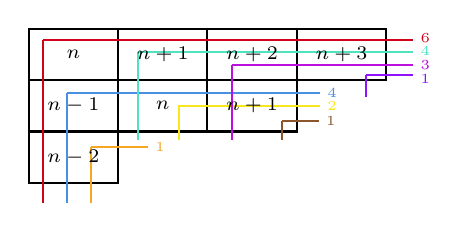
\begin{tikzpicture}[x=0.75pt,y=0.75pt,yscale=-1,xscale=1]
	%uncomment if require: \path (0,91); %set diagram left start at 0, and has height of 91
	
	%Shape: Rectangle [id:dp8815777045687874] 
	\draw   (231,3.2) -- (274.06,3.2) -- (274.06,27.97) -- (231,27.97) -- cycle ;
	%Shape: Rectangle [id:dp5991219333253064] 
	\draw   (274.06,3.2) -- (317.11,3.2) -- (317.11,27.97) -- (274.06,27.97) -- cycle ;
	%Shape: Rectangle [id:dp045704656972568536] 
	\draw   (317.11,3.2) -- (360.17,3.2) -- (360.17,27.97) -- (317.11,27.97) -- cycle ;
	%Shape: Rectangle [id:dp9709748524524378] 
	\draw   (360.17,3.2) -- (403.22,3.2) -- (403.22,27.97) -- (360.17,27.97) -- cycle ;
	%Shape: Rectangle [id:dp2596405378230242] 
	\draw   (231,27.97) -- (274.06,27.97) -- (274.06,52.73) -- (231,52.73) -- cycle ;
	%Shape: Rectangle [id:dp42226610658689956] 
	\draw   (274.06,27.97) -- (317.11,27.97) -- (317.11,52.73) -- (274.06,52.73) -- cycle ;
	%Shape: Rectangle [id:dp4187316025482162] 
	\draw   (317.11,27.97) -- (360.17,27.97) -- (360.17,52.73) -- (317.11,52.73) -- cycle ;
	%Shape: Rectangle [id:dp5305320625060379] 
	\draw   (231,52.73) -- (274.06,52.73) -- (274.06,77.49) -- (231,77.49) -- cycle ;
	%Straight Lines [id:da06952631342029836] 
	\draw [color={rgb, 255:red, 208; green, 2; blue, 27 }  ,draw opacity=1 ]   (237.87,8.48) -- (237.87,87.2) ;
	%Straight Lines [id:da009607264963725326] 
	\draw [color={rgb, 255:red, 208; green, 2; blue, 27 }  ,draw opacity=1 ]   (237.87,8.48) -- (416.31,8.48) ;
	%Straight Lines [id:da7757112780471731] 
	\draw [color={rgb, 255:red, 74; green, 144; blue, 226 }  ,draw opacity=1 ]   (249.46,34.22) -- (249.46,87.2) ;
	%Straight Lines [id:da7936647011909119] 
	\draw [color={rgb, 255:red, 74; green, 144; blue, 226 }  ,draw opacity=1 ]   (249.46,34.22) -- (371.37,34.22) ;
	%Straight Lines [id:da2080337074460996] 
	\draw [color={rgb, 255:red, 245; green, 166; blue, 35 }  ,draw opacity=1 ]   (261.04,60.31) -- (261.04,87.2) ;
	%Straight Lines [id:da1672284401195936] 
	\draw [color={rgb, 255:red, 245; green, 166; blue, 35 }  ,draw opacity=1 ]   (261.04,60.31) -- (288.56,60.31) ;
	%Straight Lines [id:da9072636327703945] 
	\draw [color={rgb, 255:red, 80; green, 227; blue, 194 }  ,draw opacity=1 ]   (283.62,14.27) -- (283.62,56.84) ;
	%Straight Lines [id:da23576145614184396] 
	\draw [color={rgb, 255:red, 80; green, 227; blue, 194 }  ,draw opacity=1 ]   (283.62,14.27) -- (416.31,14.27) ;
	%Straight Lines [id:da13302174297805824] 
	\draw [color={rgb, 255:red, 248; green, 231; blue, 28 }  ,draw opacity=1 ]   (303.31,40.62) -- (303.31,56.84) ;
	%Straight Lines [id:da18353762508780203] 
	\draw [color={rgb, 255:red, 248; green, 231; blue, 28 }  ,draw opacity=1 ]   (303.04,40.62) -- (371.37,40.62) ;
	%Straight Lines [id:da18141605076501444] 
	\draw [color={rgb, 255:red, 139; green, 87; blue, 42 }  ,draw opacity=1 ]   (353.11,47.57) -- (353.11,56.8) ;
	%Straight Lines [id:da4919198143241954] 
	\draw [color={rgb, 255:red, 139; green, 87; blue, 42 }  ,draw opacity=1 ]   (353.11,47.57) -- (370.79,47.57) ;
	%Straight Lines [id:da4333346176137032] 
	\draw [color={rgb, 255:red, 189; green, 16; blue, 224 }  ,draw opacity=1 ]   (328.79,20.64) -- (328.79,56.8) ;
	%Straight Lines [id:da4927197010903921] 
	\draw [color={rgb, 255:red, 189; green, 16; blue, 224 }  ,draw opacity=1 ]   (328.79,20.64) -- (416.31,20.64) ;
	%Straight Lines [id:da1285065636768843] 
	\draw [color={rgb, 255:red, 144; green, 19; blue, 254 }  ,draw opacity=1 ]   (393.65,25.57) -- (393.65,35.99) ;
	%Straight Lines [id:da850577775142418] 
	\draw [color={rgb, 255:red, 144; green, 19; blue, 254 }  ,draw opacity=1 ]   (393.65,25.57) -- (416.31,25.57) ;
	
	
	% Text Node
	\draw (252.53,15.58) node  [font=\scriptsize]  {$n$};
	% Text Node
	\draw (295.58,15.58) node  [font=\scriptsize]  {$n+1$};
	% Text Node
	\draw (252.53,40.35) node  [font=\scriptsize]  {$n-1$};
	% Text Node
	\draw (338.64,15.58) node  [font=\scriptsize]  {$n+2$};
	% Text Node
	\draw (295.58,40.35) node  [font=\scriptsize]  {$n$};
	% Text Node
	\draw (338.64,40.35) node  [font=\scriptsize]  {$n+1$};
	% Text Node
	\draw (381.69,15.58) node  [font=\scriptsize]  {$n+3$};
	% Text Node
	\draw (252.53,65.11) node  [font=\scriptsize]  {$n-2$};
	% Text Node
	\draw (290.56,60.31) node [anchor=west] [inner sep=0.75pt]  [font=\tiny,color={rgb, 255:red, 245; green, 166; blue, 35 }  ,opacity=1 ]  {$1$};
	% Text Node
	\draw (372.79,47.57) node [anchor=west] [inner sep=0.75pt]  [font=\tiny,color={rgb, 255:red, 139; green, 87; blue, 42 }  ,opacity=1 ]  {$1$};
	% Text Node
	\draw (418.31,27.57) node [anchor=west] [inner sep=0.75pt]  [font=\tiny,color={rgb, 255:red, 144; green, 19; blue, 254 }  ,opacity=1 ]  {$1$};
	% Text Node
	\draw (373.37,40.62) node [anchor=west] [inner sep=0.75pt]  [font=\tiny,color={rgb, 255:red, 248; green, 231; blue, 28 }  ,opacity=1 ]  {$2$};
	% Text Node
	\draw (373.37,34.22) node [anchor=west] [inner sep=0.75pt]  [font=\tiny,color={rgb, 255:red, 74; green, 144; blue, 226 }  ,opacity=1 ]  {$4$};
	% Text Node
	\draw (418.31,20.64) node [anchor=west] [inner sep=0.75pt]  [font=\tiny,color={rgb, 255:red, 189; green, 16; blue, 224 }  ,opacity=1 ]  {$3$};
	% Text Node
	\draw (418.31,14) node [anchor=west] [inner sep=0.75pt]  [font=\tiny,color={rgb, 255:red, 80; green, 227; blue, 194 }  ,opacity=1 ]  {$4$};
	% Text Node
	\draw (418.31,7.48) node [anchor=west] [inner sep=0.75pt]  [font=\tiny,color={rgb, 255:red, 208; green, 2; blue, 27 }  ,opacity=1 ]  {$6$};
	
	
\end{tikzpicture}
	\caption{$S_{\boldsymbol{abcdeznt}}$对应的杨图}
	\label{fig:young tablex of S}
\end{figure}

随后我们需要计算所谓的Hook数,考虑一条从每个底部格子下方出发的线,碰到一个格子就右转,总共经过了几个格子,如图中不同颜色的线及其对应颜色所示,而Hook数就是将所有这些数字相乘。那么整个张量的独立分量的个数就是将所有格子中的含$n$表达式相乘,再除以Hook数,例如对于$S_{\boldsymbol{abcdeznt}}$,其Hook数为
\begin{equation*}
	H=\textcolor[rgb]{0.82,0.01,0.11}{6} \times \textcolor[rgb]{0.31,0.89,0.76}{4} \times \textcolor[rgb]{0.74,0.06,0.88}{3} \times \textcolor[rgb]{0.56,0.07,1}{1} \times \textcolor[rgb]{0.29,0.56,0.89}{4} \times \textcolor[rgb]{0.97,0.91,0.11}{2} \times \textcolor[rgb]{0.55,0.34,0.16}{1} \times \textcolor[rgb]{0.96,0.65,0.14}{1} =576,
\end{equation*}
那么其独立分量的个数就为
\begin{equation*}
	\frac{1}{576}( n-2)( n-1) n^{2}( n+1)^{2}( n+2)( n+3) .
\end{equation*}
对于黎曼张量,根据\ref{eq:4.19}可以画出其杨图:

\begin{figure}[h]
	\centering
	

\tikzset{every picture/.style={line width=0.75pt}} %set default line width to 0.75pt        

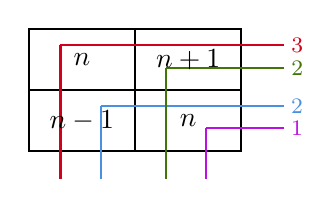
\begin{tikzpicture}[x=0.75pt,y=0.75pt,yscale=-1,xscale=1]
	%uncomment if require: \path (0,91); %set diagram left start at 0, and has height of 91
	
	%Shape: Rectangle [id:dp5303015387664369] 
	\draw   (269,15.2) -- (320.21,15.2) -- (320.21,44.66) -- (269,44.66) -- cycle ;
	%Shape: Rectangle [id:dp5868030307554879] 
	\draw   (320.21,15.2) -- (371.42,15.2) -- (371.42,44.66) -- (320.21,44.66) -- cycle ;
	%Shape: Rectangle [id:dp3019086554132011] 
	\draw   (269,44.66) -- (320.21,44.66) -- (320.21,74.11) -- (269,74.11) -- cycle ;
	%Shape: Rectangle [id:dp2331187580068521] 
	\draw   (320.21,44.66) -- (371.42,44.66) -- (371.42,74.11) -- (320.21,74.11) -- cycle ;
	%Straight Lines [id:da668298705455397] 
	\draw [color={rgb, 255:red, 208; green, 2; blue, 27 }  ,draw opacity=1 ]   (284.31,23.19) -- (284.31,87.52) ;
	%Straight Lines [id:da8368871540410545] 
	\draw [color={rgb, 255:red, 208; green, 2; blue, 27 }  ,draw opacity=1 ]   (284.31,23.19) -- (392.04,23.19) ;
	%Straight Lines [id:da20431247791258755] 
	\draw [color={rgb, 255:red, 74; green, 144; blue, 226 }  ,draw opacity=1 ]   (303.8,52.58) -- (303.8,87.52) ;
	%Straight Lines [id:da9986744066022699] 
	\draw [color={rgb, 255:red, 74; green, 144; blue, 226 }  ,draw opacity=1 ]   (303.8,52.58) -- (391.99,52.58) ;
	%Straight Lines [id:da9192673120152017] 
	\draw [color={rgb, 255:red, 65; green, 117; blue, 5 }  ,draw opacity=1 ]   (334.92,34.14) -- (334.92,87.52) ;
	%Straight Lines [id:da46108143169362115] 
	\draw [color={rgb, 255:red, 65; green, 117; blue, 5 }  ,draw opacity=1 ]   (334.92,34.14) -- (392.04,34.14) ;
	%Straight Lines [id:da40405714240560364] 
	\draw [color={rgb, 255:red, 189; green, 16; blue, 224 }  ,draw opacity=1 ]   (354.53,63.16) -- (354.53,87.56) ;
	%Straight Lines [id:da27807513919607074] 
	\draw [color={rgb, 255:red, 189; green, 16; blue, 224 }  ,draw opacity=1 ]   (354.53,63.16) -- (391.99,63.16) ;
	
	% Text Node
	\draw (294.61,29.93) node  [font=\normalsize]  {$n$};
	% Text Node
	\draw (345.82,29.93) node  [font=\normalsize]  {$n+1$};
	% Text Node
	\draw (294.61,59.38) node  [font=\normalsize]  {$n-1$};
	% Text Node
	\draw (345.82,59.38) node  [font=\normalsize]  {$n$};
	% Text Node
	\draw (393.99,63.16) node [anchor=west] [inner sep=0.75pt]  [font=\footnotesize,color={rgb, 255:red, 189; green, 16; blue, 224 }  ,opacity=1 ]  {$1$};
	% Text Node
	\draw (393.99,52.58) node [anchor=west] [inner sep=0.75pt]  [font=\footnotesize,color={rgb, 255:red, 74; green, 144; blue, 226 }  ,opacity=1 ]  {$2$};
	% Text Node
	\draw (394.04,34.14) node [anchor=west] [inner sep=0.75pt]  [font=\footnotesize,color={rgb, 255:red, 65; green, 117; blue, 5 }  ,opacity=1 ]  {$2$};
	% Text Node
	\draw (394.04,23.19) node [anchor=west] [inner sep=0.75pt]  [font=\footnotesize,color={rgb, 255:red, 208; green, 2; blue, 27 }  ,opacity=1 ]  {$3$};
	
	
\end{tikzpicture}
	\caption{$R_{\boldsymbol{abcd}}$对应的杨图}
	\label{fig:young tablex of R}
\end{figure}

那么其独立分量的个数为
\begin{equation*}
	\frac{1}{3\times 2\times 2} n^{2}( n+1)( n-1) =\frac{1}{12} n^{2} (n^{2} -1).
\end{equation*}
然而,我们谈论的“不可约性”是在$GL( n,\mathbb{C})$的框架下思考的,但如果我们考虑的是$GL( n,\mathbb{C})$的子群,那么可能会需要考虑额外的对称性。例如,我们知道对于洛伦兹群,度规$g_{\boldsymbol{ab}}$是不变量,那么这意味着这些不变量可以将张量进一步约化。最重要的例子就是我们可以将黎曼张量分成三个部分,外尔张量$C_{\boldsymbol{abcd}}$,标量曲率和无迹里奇张量(这被称为里奇分解):
\begin{equation*}
	R\boldsymbol{_{abcd}} =C\boldsymbol{_{abcd}} +E\boldsymbol{_{abcd}} +S\boldsymbol{_{abcd}} ,
\end{equation*}
其中
\begin{equation*}
	S\boldsymbol{_{abcd}} =\frac{2R}{n( n-1)} g_{\boldsymbol{a}[\boldsymbol{d}} g_{\boldsymbol{c}]\boldsymbol{b}} ,E\boldsymbol{_{abcd}} =\frac{4}{n-2} Z_{[\boldsymbol{d} |[\boldsymbol{a}} g_{\boldsymbol{b}] |\boldsymbol{c}]} ,Z_{\boldsymbol{ab}} =R_{\boldsymbol{ab}} -\frac{1}{n} Rg_{\boldsymbol{ab}} .
\end{equation*}
$C_{\boldsymbol{abcd}}$为里奇张量。这样的分解来自于所谓的无迹条件:
\begin{equation*}
	g^{\boldsymbol{ac}} C_{\boldsymbol{abcd}} =0.
\end{equation*}
如果再把洛伦兹群限制为限制性洛伦兹群,那么就会有新的不变量出现,即$e_{\boldsymbol{abcd}}$,推广的对称性会变得更复杂。这里我们考虑一个更简单的情况:
\begin{equation*}
	\phi _{\boldsymbol{ab} \cdots \boldsymbol{f}} =\phi _{\boldsymbol{AB} \cdots \boldsymbol{FA} '\boldsymbol{B} '\cdots \boldsymbol{F} '} =\phi _{(\boldsymbol{AB} \cdots \boldsymbol{F})(\boldsymbol{A} '\boldsymbol{B} '\cdots \boldsymbol{F} ')} ,
\end{equation*}
显然这里我们有
\begin{equation}
	\phi _{\boldsymbol{ab} \cdots \boldsymbol{f}} =\phi _{(\boldsymbol{ab} \cdots \boldsymbol{f})} ,\phi ^{\boldsymbol{a}}{}_{\boldsymbol{ac} \cdots \boldsymbol{f}} =0.
	\label{eq:4.20}
\end{equation}
但如果反过来我们只考虑$\phi _{\boldsymbol{ab} \cdots \boldsymbol{f}} =\phi _{(\boldsymbol{ab} \cdots \boldsymbol{f})}$一个条件,这会给出
\begin{equation*}
	\epsilon ^{\boldsymbol{AB}} \phi _{\boldsymbol{AA} '\boldsymbol{BB} '\boldsymbol{c} \cdots \boldsymbol{f}} =\epsilon ^{\boldsymbol{AB}} \phi _{\boldsymbol{BB 'AA} '\boldsymbol{c} \cdots \boldsymbol{f}} =-\epsilon ^{\boldsymbol{AB}} \phi _{\boldsymbol{AB'BA} '\boldsymbol{c} \cdots \boldsymbol{f}} ,
\end{equation*}
这意味着$\boldsymbol{A} '\boldsymbol{B} '$反对称。但根据第二个条件$\phi ^{\boldsymbol{a}}{}_{\boldsymbol{ac} \cdots \boldsymbol{f}} =0$,这意味着$\phi _{\boldsymbol{AB} \cdots \boldsymbol{FA} '\boldsymbol{B} '\cdots \boldsymbol{F} '}$在$\boldsymbol{AB} ,\boldsymbol{A} '\boldsymbol{B} '$指标上是对称的。因此我们可以看出约束一个张量的条件\ref{eq:4.20}完全等价于一个旋量的对称性。同时,如果一个复张量满足\ref{eq:4.20},我们也可以很简单地计算出复自由变量的个数,如果$\phi _{\boldsymbol{a} \cdots \boldsymbol{f}}$有$r$个指标,那么显然$\phi _{\boldsymbol{A} \cdots \boldsymbol{FA} '\cdots \boldsymbol{F} '}$有$( r+1)^{2}$个独立分量(因为具体指标$A\cdots F$只能取两个值,而对称的条件下只有$r+1$种情况)。同理,我们也可以给出以下定理:

\begin{them}[label={dof of symmetric spinor}]{对称旋量的自由度}
	如果$\varphi _{\boldsymbol{A} \cdots \boldsymbol{CP} '\cdots \boldsymbol{R} '}$是对称的并且其类型为$\{( 0,p) ,( 0,q)\}$,那么它有$( p+1)( q+1)$个(复)独立分量。
\end{them}


\section{旋量操作的张量表示}

我们已经从旋量构造出了张量,那么张量操作很显然可以被看成某些特殊的旋量操作。从这个角度看,部分旋量操作可能没有张量对应,例如单个旋量指标的缩并,或者单个旋量指标的交换。但实际上,本节我们会证明,每一个旋量操作或旋量方程都可以被写成张量操作或张量方程,但有时可能会有一些符号上的模糊性。同时,另一个非常重要的一点是,如果我们把线性旋量方程翻译成张量方程,有可能得到非线性的张量方程。


\subsection{迹反转}

我们首先考虑一些特殊情况。考察任意一个$( 0,2)$型对称张量:
\begin{equation*}
	T_{\boldsymbol{ab}} =T_{\boldsymbol{ba}} ,
\end{equation*}
旋量形式下,我们有:
\begin{equation}
	T_{\boldsymbol{AA} '\boldsymbol{BB} '} =T_{\boldsymbol{BB} '\boldsymbol{AA} '} ,
	\label{eq:4.21}
\end{equation}
这等价于
\begin{equation*}
	T_{\boldsymbol{ABA} '\boldsymbol{B} '} =\frac{1}{2}( T_{\boldsymbol{ABA} '\boldsymbol{B} '} +T_{\boldsymbol{ABB} '\boldsymbol{A} '}) +\frac{1}{2}( T_{\boldsymbol{BAB} '\boldsymbol{A} '} -T_{\boldsymbol{ABB} '\boldsymbol{A} '}) =T_{\boldsymbol{AB}(\boldsymbol{A} '\boldsymbol{B} ')} +T_{[\boldsymbol{BA}]\boldsymbol{B} '\boldsymbol{A} '} ,
\end{equation*}
而根据\ref{eq:4.21},我们知道
\begin{equation*}
	\frac{1}{2}( T_{\boldsymbol{ABA} '\boldsymbol{B} '} +T_{\boldsymbol{ABB} '\boldsymbol{A} '}) =\frac{1}{2}( T_{\boldsymbol{BAB} '\boldsymbol{A} '} +T_{\boldsymbol{ABB} '\boldsymbol{A} '}) =T_{(\boldsymbol{AB})\boldsymbol{A} '\boldsymbol{B} '} ,
\end{equation*}
这意味着
\begin{equation*}
	T_{\boldsymbol{AB}(\boldsymbol{A} '\boldsymbol{B} ')} =T_{(\boldsymbol{AB})\boldsymbol{A} '\boldsymbol{B} '} =T_{(\boldsymbol{AB})(\boldsymbol{A} '\boldsymbol{B} ')} \equiv S_{\boldsymbol{ABA} '\boldsymbol{B} '} .
\end{equation*}
同理,$T_{[\boldsymbol{BA}]\boldsymbol{B} '\boldsymbol{A} '} =T_{[\boldsymbol{BA}][\boldsymbol{B} '\boldsymbol{A} ']}$,利用等式
\begin{equation*}
	\phi _{\mathcal{D}\boldsymbol{AB}} -\phi _{\mathcal{D}\boldsymbol{BA}} =\phi {_{\mathcal{D}\boldsymbol{C}}}^{\boldsymbol{C}} \epsilon _{\boldsymbol{AB}} ,
\end{equation*}
我们可以给出
\begin{equation*}
	T_{\boldsymbol{ab}} =T_{\boldsymbol{AA} '\boldsymbol{BB} '} =S_{\boldsymbol{ABA} '\boldsymbol{B} '} +\epsilon _{\boldsymbol{AB}} \epsilon _{\boldsymbol{A} '\boldsymbol{B} '} \tau ,
\end{equation*}
其中
\begin{equation*}
	\tau =\frac{1}{4} T{_{\boldsymbol{CC} '}}^{\boldsymbol{CC} '} =\frac{1}{4} T{_{\boldsymbol{c}}}^{\boldsymbol{c}} .
\end{equation*}
这意味着我们可以将对称张量分解为
\begin{equation*}
	T_{\boldsymbol{ab}} =S_{\boldsymbol{ab}} +g_{\boldsymbol{ab}} \tau .
\end{equation*}
显然,根据\ref{eq:4.20},$S_{\boldsymbol{ab}}$是对称且无迹的,因此我们称$S_{\boldsymbol{ab}}$为$T_{\boldsymbol{ab}}$的无迹部分:
\begin{equation*}
	S_{\boldsymbol{ab}} =T_{\boldsymbol{ab}} -\frac{1}{4} g_{\boldsymbol{ab}} T{_{\boldsymbol{c}}}^{\boldsymbol{c}} .
\end{equation*}
我们称这样的操作为\textbf{迹反转}(trace reversal):
\begin{equation*}
	\hat{T}_{\boldsymbol{ab}} \equiv T_{\boldsymbol{ab}} -\frac{1}{2} g_{\boldsymbol{ab}} T{_{\boldsymbol{c}}}^{\boldsymbol{c}} ,
\end{equation*}
那么
\begin{equation*}
	\hat{T}{_{\boldsymbol{c}}}^{\boldsymbol{c}} =T{_{\boldsymbol{c}}}^{\boldsymbol{c}} -\frac{1}{2} g_{\boldsymbol{ab}} g^{\boldsymbol{ab}} T{_{\boldsymbol{c}}}^{\boldsymbol{c}} =-T{_{\boldsymbol{c}}}^{\boldsymbol{c}} .
\end{equation*}
在旋量形式中:
\begin{equation*}
	\begin{aligned}
		\hat{T}_{\boldsymbol{ab}} =\hat{T}_{\boldsymbol{AA} '\boldsymbol{BB} '} & =S_{\boldsymbol{ABA} '\boldsymbol{B} '} -\epsilon _{\boldsymbol{AB}} \epsilon _{\boldsymbol{A} '\boldsymbol{B} '} \tau \\
		& =S_{\boldsymbol{BAA} '\boldsymbol{B} '} +\epsilon _{\boldsymbol{BA}} \epsilon _{\boldsymbol{A} '\boldsymbol{B} '} \tau =T_{\boldsymbol{BAA} '\boldsymbol{B} '} =T_{\boldsymbol{ABB} '\boldsymbol{A} '} ,
	\end{aligned}
\end{equation*}
这意味着某两个旋量指标交换位置等价于(对称)张量上的迹反转操作。


\subsection{对偶化}

现在考虑任意一个反对称的$( 0,2)$类的世界张量,有时候也被称为双矢(bivector):
\begin{equation*}
	F_{\boldsymbol{ab}} =-F_{\boldsymbol{ba}} ,
\end{equation*}
旋量形式中这意味着
\begin{equation*}
	F_{\boldsymbol{AA} '\boldsymbol{BB} '} =-F_{\boldsymbol{BB} '\boldsymbol{AA} '} ,
\end{equation*}
这意味着
\begin{equation}
	F_{\boldsymbol{ABA} '\boldsymbol{B} '} =\frac{1}{2}( F_{\boldsymbol{ABA} '\boldsymbol{B} '} -T_{\boldsymbol{ABB} '\boldsymbol{A} '}) +\frac{1}{2}( F_{\boldsymbol{ABB} '\boldsymbol{A} '} -F_{\boldsymbol{BAB} '\boldsymbol{A} '}) =\phi _{\boldsymbol{AB}} \epsilon _{\boldsymbol{A'B} '} +\epsilon _{\boldsymbol{AB}} \psi _{\boldsymbol{A} '\boldsymbol{B} '} ,
	\label{eq:4.22}
\end{equation}
其中
\begin{equation*}
	\phi _{\boldsymbol{AB}} =\phi _{(\boldsymbol{AB})} =\frac{1}{2} F{_{\boldsymbol{ABC} '}}^{\boldsymbol{C} '} ,\psi _{\boldsymbol{A} '\boldsymbol{B} '} =\psi _{(\boldsymbol{A} '\boldsymbol{B} ')} =\frac{1}{2} F{_{\boldsymbol{C}}}^{\boldsymbol{C}}{}_{\boldsymbol{A} '\boldsymbol{B} '} .
\end{equation*}
如果对\ref{eq:4.22}取复共轭,我们有
\begin{equation*}
	\overline{F}_{\boldsymbol{ab}} =\overline{F}_{\boldsymbol{A} '\boldsymbol{B} '\boldsymbol{AB}} =\overline{\phi }_{\boldsymbol{A} '\boldsymbol{B} '} \epsilon _{\boldsymbol{AB}} +\epsilon _{\boldsymbol{A} '\boldsymbol{B} '}\overline{\psi }_{\boldsymbol{AB}} ,
\end{equation*}
这意味着复共轭操作$F_{\boldsymbol{ab}} \mapsto \overline{F}_{\boldsymbol{ab}}$对应$\psi _{\boldsymbol{A} '\boldsymbol{B} '} \mapsto \overline{\phi }_{\boldsymbol{A} '\boldsymbol{B} '}$。那么如果$F_{\boldsymbol{ab}}$是实的,这意味着$\psi _{\boldsymbol{A} '\boldsymbol{B} '} =\overline{\phi }_{\boldsymbol{A} '\boldsymbol{B} '}$,或
\begin{equation}
	F_{\boldsymbol{ab}} =\phi _{\boldsymbol{AB}} \epsilon _{\boldsymbol{A'B} '} +\epsilon _{\boldsymbol{AB}}\overline{\phi }_{\boldsymbol{A} '\boldsymbol{B} '} ,
	\label{eq:4.23}
\end{equation}
这意味着实反对称$F_{\boldsymbol{ab}}$与对称旋量$\phi _{\boldsymbol{AB}}$有一一对应关系。



现在我们定义$F_{\boldsymbol{ab}}$的对偶$\prescript{*}{}{} F_{\boldsymbol{ab}}$为
\begin{equation*}
	\prescript{*}{}{} F_{\boldsymbol{ab}} =\frac{1}{2} e_{\boldsymbol{abcd}} F^{\boldsymbol{cd}} =\frac{1}{2} e{_{\boldsymbol{ab}}}^{\boldsymbol{cd}} F_{\boldsymbol{cd}} .
\end{equation*}
那么如果我们将$e_{\boldsymbol{abcd}}$的定义\ref{eq:4.16}带入\ref{eq:4.22},可以给出
\begin{equation}
	\prescript{*}{}{} F_{\boldsymbol{ab}} =\prescript{*}{}{} F_{\boldsymbol{ABA} '\boldsymbol{B} '} =-\mathrm{i} \phi _{\boldsymbol{AB}} \epsilon _{\boldsymbol{A} '\boldsymbol{B} '} +\mathrm{i} \epsilon _{\boldsymbol{AB}} \psi _{\boldsymbol{A} '\boldsymbol{B} '} ,
	\label{eq:4.24}
\end{equation}
即
\begin{equation*}
	\prescript{*}{}{} F_{\boldsymbol{ABA} '\boldsymbol{B} '} =\mathrm{i} F_{\boldsymbol{ABB} '\boldsymbol{A} '} =-\mathrm{i} F_{\boldsymbol{BAA} '\boldsymbol{B} '} ,
\end{equation*}
这意味着对于反对称张量,旋量指标的置换等于将其代换成$\pm \mathrm{i}$乘其对偶$\prescript{*}{}{} F$!那么将指标置换两次,自然得到
\begin{equation*}
	\prescript{**}{}{} F_{\boldsymbol{ab}} =F_{\boldsymbol{ba}} =-F_{\boldsymbol{ab}} .
\end{equation*}
考虑更一般的情况,对于一个大张量中的两个反对称指标取对偶:
\begin{equation*}
	\prescript{*}{}{} G_{\boldsymbol{ab}\mathcal{A}} \equiv \frac{1}{2} e{_{\boldsymbol{ab}}}^{\boldsymbol{cd}} G_{\boldsymbol{cd}\mathcal{A}} ,G_{\boldsymbol{ab}\mathcal{A}} =G_{[\boldsymbol{ab}]\mathcal{A}} .
\end{equation*}
我们给出一个有用的引理:
\begin{equation}
	\prescript{*}{}{} G_{[\boldsymbol{abc}]\mathcal{A}} =0\Leftrightarrow \prescript{*}{}{} G^{\boldsymbol{ab}}{}_{\boldsymbol{a}\mathcal{A}} =0.
	\label{eq:4.25}
\end{equation}
要证明这个只需注意到
\begin{equation*}
	G_{[\boldsymbol{abc}]\mathcal{A}} =g{_{[\boldsymbol{a}}}^{\boldsymbol{p}} g{_{\boldsymbol{b}}}^{\boldsymbol{q}} g{_{\boldsymbol{c}]}}^{\boldsymbol{r}} G_{\boldsymbol{pqr}\mathcal{A}} =-\frac{1}{6} e_{\boldsymbol{abcd}} e^{\boldsymbol{pqrd}} G_{\boldsymbol{pqr}\mathcal{A}} =\frac{1}{3} e_{\boldsymbol{abcd}}\prescript{*}{}{} G^{\boldsymbol{pd}}{}_{\boldsymbol{p}\mathcal{A}} ,
\end{equation*}
因此如果$\prescript{*}{}{} G^{\boldsymbol{pd}}{}_{\boldsymbol{p}\mathcal{A}} =0\Rightarrow G_{[\boldsymbol{abc}]\mathcal{A}} \Rightarrow \prescript{*}{}{} G_{[\boldsymbol{abc}]\mathcal{A}} =0$。反过来,注意到
\begin{equation*}
	\begin{aligned}
		& \prescript{*}{}{} G^{\boldsymbol{ab}}{}_{\boldsymbol{f}\mathcal{A}} =\frac{1}{2} e^{\boldsymbol{abcd}} G_{\boldsymbol{cdf}\mathcal{B}} =\frac{1}{2} e^{\boldsymbol{abcd}} G_{[\boldsymbol{fcd}]\mathcal{A}}\\
		\Rightarrow  & \prescript{*}{}{} G_{[\boldsymbol{abf}]\mathcal{A}} =\frac{1}{2} e{_{\boldsymbol{ab}}}^{\boldsymbol{cd}} G_{[\boldsymbol{fcd}]\mathcal{A}} =0\\
		\Rightarrow  & \prescript{*}{}{} G^{\boldsymbol{ab}}{}_{\boldsymbol{f}\mathcal{A}} =0.
	\end{aligned}
\end{equation*}
对于一个指标或者三个指标反对称的情况,也可以构造对偶:
\begin{equation*}
	\prescript{\dagger }{}{} J_{\boldsymbol{abc}\mathcal{A}} \equiv e{_{\boldsymbol{abc}}}^{\boldsymbol{d}} J_{\boldsymbol{d}\mathcal{A}} ,\prescript{\ddagger }{}{} K_{\boldsymbol{a}\mathcal{B}} \equiv \frac{1}{6} e{_{\boldsymbol{a}}}^{\boldsymbol{bcd}} K_{\boldsymbol{bcd}\mathcal{B}} ,
\end{equation*}
容易证明
\begin{equation*}
	\prescript{\dagger \ddagger }{}{} J_{\boldsymbol{a}\mathcal{A}} =J_{\boldsymbol{a}\mathcal{A}} ,\prescript{\ddagger \dagger }{}{} K_{\boldsymbol{abc}\mathcal{B}} =K_{\boldsymbol{abc}\mathcal{B}} .
\end{equation*}
如果将$\mathcal{A}$换为$\boldsymbol{d}\mathcal{C}$,将$\mathcal{B}$换位$\boldsymbol{d}\mathcal{D}$,我们容易证明
\begin{equation*}
	\prescript{\dagger }{}{} J_{[\boldsymbol{abcd}]\mathcal{C}} =\frac{1}{4} e_{\boldsymbol{abcd}} J{_{\boldsymbol{f}}}^{\boldsymbol{f}}{}_{\mathcal{C}} ,K_{[\boldsymbol{abcd}]\mathcal{D}} =\frac{1}{4} e_{\boldsymbol{abcd}}\prescript{\ddagger }{}{} K{_{\boldsymbol{f}}}^{\boldsymbol{f}}{}_{\mathcal{D}} .
\end{equation*}
旋量形式中,我们带入直接带入$e$的定义可以给出
\begin{equation*}
	\begin{aligned}
		\prescript{\dagger }{}{} J_{\boldsymbol{abc}\mathcal{A}} & =\mathrm{i} \epsilon _{\boldsymbol{AC}} \epsilon _{\boldsymbol{B} '\boldsymbol{C} '} J_{\boldsymbol{BA} '\mathcal{A}} -\mathrm{i} \epsilon _{\boldsymbol{BC}} \epsilon _{\boldsymbol{A} '\boldsymbol{C} '} J_{\boldsymbol{AB} '\mathcal{A}} ,\\
		\prescript{\ddagger }{}{} K_{\boldsymbol{a}\mathcal{B}} & =\frac{\mathrm{i}}{3} K{_{\boldsymbol{AB} '\boldsymbol{BA} '}}^{\boldsymbol{BB} '}{}_{\mathcal{B}} .
	\end{aligned}
\end{equation*}
现在我们回到$F_{\boldsymbol{ab}}$。考虑两种情况:
\begin{enumerate}[label=(\alph*)]
	\item $\prescript{*}{}{} F_{\boldsymbol{ab}} =-\mathrm{i} F_{\boldsymbol{ab}}$,等价于$F_{\boldsymbol{ABA} '\boldsymbol{B} '} =F_{\boldsymbol{BAA} '\boldsymbol{B} '} =-F_{\boldsymbol{ABB} '\boldsymbol{A} '}$,即$F_{\boldsymbol{ABA} '\boldsymbol{B} '} =F_{(\boldsymbol{AB})[\boldsymbol{A} '\boldsymbol{B} ']}$。我们称这种情况为自对偶的。
	\item $\prescript{*}{}{} F_{\boldsymbol{ab}} =\mathrm{i} F_{\boldsymbol{ab}}$,等价于$F_{\boldsymbol{ABA} '\boldsymbol{B} '} =-F_{\boldsymbol{BAA} '\boldsymbol{B} '} =F_{\boldsymbol{ABB} '\boldsymbol{A} '}$,即$F_{\boldsymbol{ABA} '\boldsymbol{B} '} =F_{[\boldsymbol{AB}](\boldsymbol{A} '\boldsymbol{B} ')}$。我们称这种情况为反自对偶的。
\end{enumerate}

我们从\ref{eq:4.22},\ref{eq:4.24}中可以给出,任何一个反对称张量都可以被分解为:
\begin{equation*}
	F_{\boldsymbol{ab}} =\prescript{-}{}{} F_{\boldsymbol{ab}} +\prescript{+}{}{} F_{\boldsymbol{ab}}
\end{equation*}
其中
\begin{equation*}
	\begin{aligned}
		\prescript{-}{}{} F_{\boldsymbol{ab}} & \equiv \frac{1}{2} (F_{\boldsymbol{ab}} +\mathrm{i}\prescript{*}{}{} F_{\boldsymbol{ab}} )=\phi _{\boldsymbol{AB}} \epsilon _{\boldsymbol{A'B} '}\\
		\prescript{+}{}{} F_{\boldsymbol{ab}} & \equiv \frac{1}{2} (F_{\boldsymbol{ab}} -\mathrm{i}\prescript{*}{}{} F_{\boldsymbol{ab}} )=\epsilon _{\boldsymbol{AB}} \psi _{\boldsymbol{A} '\boldsymbol{B} '} ,
	\end{aligned}
\end{equation*}
而$\prescript{-}{}{} F$是反自对偶的,$\prescript{+}{}{} F$是自对偶的。



如果将对偶操作推广,可得到操作\textbf{对偶性旋转}(duality rotation),$F_{\boldsymbol{ab}} \mapsto \prescript{( \theta )}{}{} F_{\boldsymbol{ab}}$,定义为
\begin{equation*}
	\prescript{( \theta )}{}{} F_{\boldsymbol{ab}} \equiv F_{\boldsymbol{ab}}\cos \theta +\prescript{*}{}{} F_{\boldsymbol{ab}}\sin \theta =\prescript{-}{}{} F_{\boldsymbol{ab}}\mathrm{e}^{-\mathrm{i} \theta } +\prescript{+}{}{} F_{\boldsymbol{ab}}\mathrm{e}^{\mathrm{i} \theta } =\mathrm{e}^{-\mathrm{i} \theta } \phi _{\boldsymbol{AB}} \epsilon _{\boldsymbol{A} '\boldsymbol{B} '} +\mathrm{e}^{\mathrm{i} \theta } \epsilon _{\boldsymbol{AB}} \psi _{\boldsymbol{A} '\boldsymbol{B} '} .
\end{equation*}


我们可以用旋量证明许多(反)自对偶矢量的性质,例如对于任意两个张量$F,G$,都有
\begin{equation*}
	\prescript{-}{}{} F_{\boldsymbol{ab}}\prescript{+}{}{} G^{\boldsymbol{ab}} =0,\prescript{-}{}{} F{_{\boldsymbol{a}}}^{\boldsymbol{b}}\prescript{+}{}{} G_{\boldsymbol{bc}} =\prescript{+}{}{} G{_{\boldsymbol{a}}}^{\boldsymbol{b}}\prescript{-}{}{} F_{\boldsymbol{bc}} .
\end{equation*}
只需要带入计算即可,但是后者对于张量方法证明则较为麻烦。


\subsection{一般转换流程}

我们已经看到,对于一个对称张量,交换其旋量指标等价于将其变换成迹反转,而对于一个反对称张量,交换其旋量指标等价于将其变换成对偶,那么对于一个一般的$( 0,2)$型张量$H_{\boldsymbol{ab}}$,我们知道
\begin{equation*}
	H_{\boldsymbol{AA} '\boldsymbol{BB} '} =H_{(\boldsymbol{ab})} +H_{[\boldsymbol{ab}]} ,
\end{equation*}
那么交换指标给出
\begin{equation*}
	\begin{aligned}
		H_{\boldsymbol{BAA} '\boldsymbol{B} '} & =\hat{H}_{(\boldsymbol{ab})} +\mathrm{i}\prescript{*}{}{} H_{[\boldsymbol{ab}]} =\frac{1}{2} (H_{\boldsymbol{ab}} +H_{\boldsymbol{ba}} -H{_{\boldsymbol{c}}}^{\boldsymbol{c}} g_{\boldsymbol{ab}} +\mathrm{i} e_{\boldsymbol{abcd}} H^{\boldsymbol{cd}} ),\\
		H_{\boldsymbol{ABB} '\boldsymbol{A} '} & =\hat{H}_{(\boldsymbol{ab})} -\mathrm{i}\prescript{*}{}{} H_{[\boldsymbol{ab}]} =\frac{1}{2} (H_{\boldsymbol{ab}} +H_{\boldsymbol{ba}} -H{_{\boldsymbol{c}}}^{\boldsymbol{c}} g_{\boldsymbol{ab}} -\mathrm{i} e_{\boldsymbol{abcd}} H^{\boldsymbol{cd}} ).
	\end{aligned}
\end{equation*}
由于交换旋量指标完全可以通过旋量度规升降指标实现,这意味着我们也可以构造一个算符完成这件事。一个自然的构造是
\begin{equation*}
	\begin{aligned}
		U{_{\boldsymbol{ab}}}^{\boldsymbol{cd}} & =\epsilon {_{\boldsymbol{A}}}^{\boldsymbol{D}} \epsilon {_{\boldsymbol{B}}}^{\boldsymbol{C}} \epsilon {_{\boldsymbol{A} '}}^{\boldsymbol{C} '} \epsilon {_{\boldsymbol{B} '}}^{\boldsymbol{D} '}\\
		& =\frac{1}{2} (g{_{\boldsymbol{a}}}^{\boldsymbol{c}} g{_{\boldsymbol{b}}}^{\boldsymbol{d}} +g{_{\boldsymbol{a}}}^{\boldsymbol{d}} g{_{\boldsymbol{b}}}^{\boldsymbol{c}} -g_{\boldsymbol{ab}} g^{\boldsymbol{cd}} +\mathrm{i} e{_{\boldsymbol{ab}}}^{\boldsymbol{cd}} ),
	\end{aligned}
\end{equation*}
那么旋量指标的交换自然为
\begin{equation*}
	H_{\boldsymbol{BAA} '\boldsymbol{B} '} =U{_{\boldsymbol{ab}}}^{\boldsymbol{cd}} H_{\boldsymbol{cd}} ,H_{\boldsymbol{ABB} '\boldsymbol{A} '} =\overline{U}{_{\boldsymbol{ab}}}^{\boldsymbol{cd}} H_{\boldsymbol{cd}} .
\end{equation*}
同时注意到
\begin{equation*}
	U^{\boldsymbol{ab}}{}_{\boldsymbol{cd}} =U{_{\boldsymbol{cd}}}^{\boldsymbol{ab}} ,U{_{\boldsymbol{ba}}}^{\boldsymbol{cd}} =\overline{U}{_{\boldsymbol{ab}}}^{\boldsymbol{cd}} =U{_{\boldsymbol{ab}}}^{\boldsymbol{dc}} ,
\end{equation*}
那么我们可以写出
\begin{equation*}
	H^{\boldsymbol{BAA} '\boldsymbol{B} '} =U{_{\boldsymbol{cd}}}^{\boldsymbol{ab}} H^{\boldsymbol{cd}} ,H_{\boldsymbol{ABB} '\boldsymbol{A} '} =U{_{\boldsymbol{ba}}}^{\boldsymbol{cd}} H_{\boldsymbol{cd}} .
\end{equation*}
因此,用这个算符$U$我们可以将\textbf{任何}旋量指标替换变成旋量形式,因为任何指标代换可以被写成旋量指标交换的复合。



最后我们讨论如何将一个一般的旋量$\chi _{\mathcal{A}} =\chi _{\boldsymbol{A} \cdots \boldsymbol{EB} '\cdots \boldsymbol{F} '}$给出其张量实现。我们分为三种情况:
\begin{itemize}
	\item 如果带撇与不带撇的指标数一样,那么我们只需要使用指标替换操作,将带撇的指标替换成与不带撇的指标一样的指标,给出其张量版本。但我们知道,指标替换的方式不止一种,例如我们可以让$\chi _{\boldsymbol{ABCD} '\boldsymbol{E} '\boldsymbol{F} '} \mapsto \chi _{\boldsymbol{ABCA} '\boldsymbol{B} '\boldsymbol{C} '}$,但也可以将其换为$\chi _{\boldsymbol{ABCB} '\boldsymbol{A} '\boldsymbol{C} '}$,或$\chi _{\boldsymbol{EBDB} '\boldsymbol{E} '\boldsymbol{D} '}$。然而我们知道,这样做的区别仅仅在于旋量指标的位置有置换,而这对应于相应的张量算符$U$,因此我们只需要选择其中一个,其他张量实现都与选择的张量相差一个张量变换。
	\item 如果旋量指标的总数是偶数,即使带撇和不带撇的指标数可能不一样。那么这种情况,我们只需要将其乘以$\epsilon $张量,将不足的指标补齐,便可回到第一种情况,并且这样做也没有添加任何信息。例如对于旋量$\psi _{\boldsymbol{AB}} ,\phi _{\boldsymbol{AB} '\boldsymbol{C} '\boldsymbol{D} '}$,我们可以将其张量实现选为$P_{\boldsymbol{ab}} =\psi _{\boldsymbol{AB}} \epsilon _{\boldsymbol{A} '\boldsymbol{B} '}$,以及$Q_{\boldsymbol{abc}} =\phi _{\boldsymbol{AA} '\boldsymbol{B} '\boldsymbol{C} '} \epsilon _{\boldsymbol{BC}}$。
	\item 如果旋量指标的总数是奇数,这种情况无法完全用张量实现,可能会有一个符号的不确定性。接受了这点,我们只需要用$\chi _{\mathcal{A}_{1}} \chi _{\mathcal{A}_{2}}$,这样就能将$\chi _{\mathcal{A}}$确定到一个符号的差距。例如对于旋量$\kappa _{\boldsymbol{A}}$,我们首先将其“平方”得到$\kappa _{\boldsymbol{A}} \kappa _{\boldsymbol{B}}$,随后乘以$\epsilon _{\boldsymbol{A} '\boldsymbol{B} '}$。为了几何上的实现方便,我们可以构造$P_{\boldsymbol{ab}} =\kappa _{\boldsymbol{A}} \kappa _{\boldsymbol{B}} \epsilon _{\boldsymbol{A} '\boldsymbol{B} '} +\epsilon _{\boldsymbol{AB}}\overline{\kappa }_{\boldsymbol{A} '}\overline{\kappa }_{\boldsymbol{B} '}$。实际上,这就是我们之前给出的\ref{eq:4.13}。
\end{itemize}


\section{流形上某点的张量和旋量*}

本节我们给出一些对于在流形上某点的旋量成立的结论,这意味着这些结论可能对于流形上的旋量场并不成立。有些定理我们不会给出证明,仅仅罗列结论。

\begin{them}[label={them:3.5}]{}
	如果$\psi _{\mathcal{A}} \phi _{\mathcal{B}} =\chi _{\mathcal{A}} \theta _{\mathcal{B}} \neq 0$,那么$\psi _{\mathcal{A}} =\kappa \chi _{\mathcal{A}}$,且$\phi _{\mathcal{B}} =\kappa ^{-1} \theta _{\mathcal{B}}$,其中$\kappa \in \mathfrak{S}$非零。
\end{them}

\begin{proof}
	选取一个$\xi ^{\mathcal{B}}$在等式两边缩并给出$\psi _{\mathcal{A}} \phi _{\mathcal{B}} \xi ^{\mathcal{B}} =\chi _{\mathcal{A}} \theta _{\mathcal{B}} \xi ^{\mathcal{B}}$,选取$\xi $令$\lambda \equiv \phi _{\mathcal{B}} \xi ^{\mathcal{B}} \neq 0$,那么我们知道
	\begin{equation*}
		\psi _{\mathcal{A}} =\kappa \chi _{\mathcal{A}} ,\kappa =\lambda ^{-1} \theta _{\mathcal{B}} \xi ^{\mathcal{B}} .
	\end{equation*}
	同理$\phi _{\mathcal{B}} =\kappa ^{-1} \theta _{\mathcal{B}}$。
\end{proof}

\begin{them}[label={them:3.6}]{}
	如果$\psi _{\mathcal{AB}} \phi _{\mathcal{CD}} =\chi _{\mathcal{AD}} \theta _{\mathcal{CB}} \neq 0$,那么存在$\alpha _{\mathcal{A}} ,\beta _{\mathcal{B}} ,\gamma _{\mathcal{C}} ,\rho _{\mathcal{D}}$,使得
	\begin{equation*}
		\psi _{\mathcal{AB}} =\alpha _{\mathcal{A}} \beta _{\mathcal{B}} ,\phi _{\mathcal{CD}} =\gamma _{\mathcal{C}} \rho _{\mathcal{D}} ,\chi _{\mathcal{AD}} =\alpha _{\mathcal{A}} \rho _{\mathcal{D}} ,\theta _{\mathcal{CB}} =\gamma _{\mathcal{C}} \beta _{\mathcal{B}} .
	\end{equation*}
\end{them}

\begin{proof}
	思路同上,选取$\xi ^{\mathcal{C}} ,\eta ^{\mathcal{D}}$令$\lambda \equiv \xi ^{\mathcal{C}} \eta ^{\mathcal{D}} \phi _{\mathcal{CD}} \neq 0$,那么两边取内积给出$\psi _{\mathcal{AB}} \lambda =(\chi _{\mathcal{AD}} \eta ^{\mathcal{D}} )(\xi ^{\mathcal{C}} \theta _{\mathcal{CB}} )$。只需令$\alpha _{\mathcal{A}} =\lambda ^{-1} \chi _{\mathcal{AD}} \eta ^{\mathcal{D}}$,$\beta _{\mathcal{B}} =\xi ^{\mathcal{C}} \theta _{\mathcal{CB}}$,那么我们有$\psi _{\mathcal{AB}} =\alpha _{\mathcal{A}} \beta _{\mathcal{B}}$。同理可得其他部分。
\end{proof}

作为上述定理的一个特殊情况,我们看到如果$\psi _{[\mathcal{A}_{1}} \phi _{\mathcal{A}_{2}]} =0$,那么$\psi _{\mathcal{A}} =\kappa \phi _{\mathcal{A}}$或$\phi _{\mathcal{A}} =0$。

\begin{them}[label={them:3.7}]{}
	对于$\lambda {_{\mathcal{AB}}}^{\mathcal{Q}}$,以下三个条件等价:
	\begin{enumerate}[label=(\alph*)]
		\item $\lambda {_{\mathcal{AB}}}^{\mathcal{Q}} \xi _{\mathcal{Q}}$对于每一个$\xi _{\mathcal{Q}} \in \mathfrak{S}_{\mathcal{Q}}$可以写成$\rho _{\mathcal{A}} \zeta _{\mathcal{B}}$的形式。
		\item $\lambda {_{\mathcal{A}_{1}[\mathcal{B}_{1}}}^{(\mathcal{Q}_{1}} \lambda {_{|\mathcal{A}_{2} |\mathcal{B}_{2}]}}^{\mathcal{Q}_{2})} =0$。
		\item $\lambda {_{\mathcal{AB}}}^{\mathcal{Q}}$可以被写成要么$\alpha _{\mathcal{A}} \phi {_{\mathcal{B}}}^{\mathcal{Q}}$的形式,要么$\theta {_{\mathcal{B}}}^{\mathcal{Q}} \beta _{\mathcal{A}}$的形式。
	\end{enumerate}
\end{them}

这个定理的证明只需将$\lambda {_{\mathcal{A}_{1}[\mathcal{B}_{1}}}^{(\mathcal{Q}_{1}} \lambda {_{|\mathcal{A}_{2} |\mathcal{B}_{2}]}}^{\mathcal{Q}_{2})} =0$展开,并适当缩并即可。

\begin{them}[label={them:3.8}]{}
	$\psi {_{(\mathcal{A}_{1} \cdots \mathcal{A}_{r}}}^{\mathcal{B}} \phi {_{\mathcal{A}_{r+1} \cdots \mathcal{A}_{r+s})}}^{\mathcal{C}} =0$意味着要么$\psi {_{(\mathcal{A}_{1} \cdots \mathcal{A}_{r})}}^{\mathcal{B}} =0$,要么$\phi {_{(\mathcal{A}_{1} \cdots \mathcal{A}_{s})}}^{\mathcal{C}} =0$。
\end{them}

\begin{proof}
	只需要考虑$\psi {_{\mathcal{A}_{1} \cdots \mathcal{A}_{r}}}^{\mathcal{B}} \xi ^{\mathcal{A}_{1}} \cdots \xi ^{\mathcal{A}_{r}} \phi {_{\mathcal{A}_{r+1} \cdots \mathcal{A}_{r+s}}}^{\mathcal{C}} \xi ^{\mathcal{A}_{r+1}} \cdots \xi ^{\mathcal{A}_{r+s}}$,随后使用\ref{them:zero symmetric spinor}以及\ref{them:3.5}即可证明。
\end{proof}


以上结果对于任意维度都适用,但对于二维的旋量空间,有些特殊的结论,例如根据\ref{them:3.6},我们知道如果$\psi _{\mathcal{A}\boldsymbol{B}} ,\theta _{\mathcal{C}\boldsymbol{B}} \neq 0$,那么$\psi {_{\mathcal{A}}}^{\boldsymbol{B}} \theta _{\mathcal{C}\boldsymbol{B}} =0$可以推出$\psi _{\mathcal{A}\boldsymbol{B}} =\alpha _{\mathcal{A}} \beta _{\boldsymbol{B}} ,\theta _{\mathcal{C}\boldsymbol{B}} =\gamma _{\mathcal{C}} \beta _{\boldsymbol{B}}$。


\subsection{主类光方向}

下面的结果除了用了自旋空间的二维性,还使用了$\mathfrak{S}$作为复数的可除环是代数上封闭的这个条件。

\begin{them}[label={them:3.9}]{}
	如果$\phi _{\boldsymbol{AB} \cdots \boldsymbol{L}} =\phi _{(\boldsymbol{AB} \cdots \boldsymbol{L})} \neq 0$,那么存在$\alpha _{\boldsymbol{A}} ,\beta _{\boldsymbol{A}} ,\cdots ,\lambda _{\boldsymbol{A}} \in \mathfrak{S}_{\boldsymbol{A}}$满足
	\begin{equation}
		\phi _{\boldsymbol{AB} \cdots \boldsymbol{L}} =\alpha _{(\boldsymbol{A}} \beta _{\boldsymbol{B}} \cdots \lambda _{\boldsymbol{L})} ,
		\label{eq:4.26}
	\end{equation}
	且这个分解在相差一个系数的意义上是唯一的。
\end{them}

\begin{proof}
	选取一个自旋标架:$o^{\boldsymbol{A}} ,\iota ^{\boldsymbol{A}}$,在这个标架下满足$\phi _{111\cdots 1} \neq 0$。同时选取一个$\xi ^{\boldsymbol{A}} \in \mathfrak{S}^{\boldsymbol{A}}$,满足在这个标架下的分量为$(\xi ^{0} ,\xi ^{1} )=( 1,z)$,那么如果$\phi $有$n$个自旋指标,我们知道
	\begin{equation*}
		\phi _{\boldsymbol{AB} \cdots \boldsymbol{L}} \xi ^{\boldsymbol{A}} \xi ^{\boldsymbol{B}} \cdots \xi ^{\boldsymbol{L}} =\phi _{00\cdots 0} +nz\phi _{10\cdots 0} +\cdots +z^{n} \phi _{11\cdots 1} ,
	\end{equation*}
	根据代数学基本定理,上述多项式一定有一个在相差常数的意义下有一个唯一的分解:
	\begin{equation*}
		\phi _{\boldsymbol{AB} \cdots \boldsymbol{L}} \xi ^{\boldsymbol{A}} \xi ^{\boldsymbol{B}} \cdots \xi ^{\boldsymbol{L}} =(\alpha _{0} +z\alpha _{1} )(\beta _{0} +z\beta _{1} )\cdots (\lambda _{0} +z\lambda _{1} ),
	\end{equation*}
	那么我们令$\alpha _{\boldsymbol{A}} =(\alpha ^{0} ,\alpha ^{1} )$,那么我们知道$\alpha _{0} +z\alpha _{1} =\alpha _{A} \xi ^{A} =\alpha _{\boldsymbol{A}} \xi ^{\boldsymbol{A}}$,从而
	\begin{equation*}
		\phi _{\boldsymbol{AB} \cdots \boldsymbol{L}} \xi ^{\boldsymbol{A}} \xi ^{\boldsymbol{B}} \cdots \xi ^{\boldsymbol{L}} =(\alpha _{\boldsymbol{A}} \xi ^{\boldsymbol{A}} )(\beta _{\boldsymbol{B}} \xi ^{\boldsymbol{B}} )\cdots (\lambda _{\boldsymbol{L}} \xi ^{\boldsymbol{L}} ),
	\end{equation*}
	因此
	\begin{equation*}
		\{\phi _{\boldsymbol{AB} \cdots \boldsymbol{L}} -\alpha _{(\boldsymbol{A}} \beta _{\boldsymbol{B}} \cdots \lambda _{\boldsymbol{L})}\} \xi ^{\boldsymbol{A}} \xi ^{\boldsymbol{B}} \cdots \xi ^{\boldsymbol{L}} =0.
	\end{equation*}
	根据\ref{them:zero symmetric spinor},我们知道有式\ref{eq:4.26}。
\end{proof}


我们将这种把对称张量分解的方法叫做\textbf{正则分解}(canonical decomposition),其中这样构造出的旋量$\alpha _{\boldsymbol{A}} ,\beta _{\boldsymbol{A}} ,\cdots ,\lambda _{\boldsymbol{L}}$被称为\textbf{主旋量}(principal spinor)。我们知道一个旗杆$K^{\boldsymbol{a}} =\kappa ^{\boldsymbol{A}}\overline{\kappa }^{\boldsymbol{A} '}$对应了很多不同的主旋量,我们称这样的方向为\textbf{主类光方向}(principal null directions, PND),其对应类光矢量被称为\textbf{主类光矢量}(principal null vectors)。因此,每一个对称的$n$指标旋量唯一地定义了$n$个PND,虽然可能会有重数,如果分解\ref{eq:4.26}给出了$k$个相同的PND,那么我们称这个PND为$k$-重($k$-fold)的。



如果$\alpha _{\boldsymbol{A}}$为$k$-重的主旋量,那么我们知道:
\begin{equation*}
	\phi _{\boldsymbol{AB} \cdots \boldsymbol{DE} \cdots \boldsymbol{L}} =\alpha _{(\boldsymbol{A}} \alpha _{\boldsymbol{B}} \cdots \alpha _{\boldsymbol{D}} \eta _{\boldsymbol{E}} \cdots \lambda _{\boldsymbol{L})} ,
\end{equation*}
其中$\eta ,\cdots \lambda $都不正比于$\alpha $,如果将对称化打开,并且与$\alpha ^{\boldsymbol{E}} \cdots \alpha ^{\boldsymbol{L}}$缩并,我们知道
\begin{equation}
	\phi _{\boldsymbol{AB} \cdots \boldsymbol{DE} \cdots \boldsymbol{L}} \alpha ^{\boldsymbol{E}} \cdots \alpha ^{\boldsymbol{L}} =\kappa \alpha _{\boldsymbol{A}} \alpha _{\boldsymbol{B}} \cdots \alpha _{\boldsymbol{D}} ,
	\label{eq:4.27}
\end{equation}
其中
\begin{equation*}
	\kappa =\frac{k!( n-k) !}{n!} (\eta _{\boldsymbol{E}} \alpha ^{\boldsymbol{E}} )\cdots (\lambda _{\boldsymbol{L}} \alpha ^{\boldsymbol{L}} )\neq 0,
\end{equation*}
如果再对\ref{eq:4.27}多用一个$\alpha $缩并,我们会得到零,因此我们给出定理:

\begin{them}[label={them:3.10}]{$k$-重主旋量成立条件}
	如果$\xi _{\boldsymbol{A}} \neq 0$是对称旋量$\phi _{\boldsymbol{AB} \cdots \boldsymbol{L}}$的一个$k$-重主旋量,那么其充要条件为$\phi _{\boldsymbol{A} \cdots \boldsymbol{L}}$与$n-k$个$\xi $的缩并不为零,但与$n-k+1$个$\xi $缩并为零。
\end{them}

\ref{them:3.10}有一个显然的推论,即对于对称旋量$\phi _{\boldsymbol{AB} \cdots \boldsymbol{L}}$,如果
\begin{equation*}
	\xi ^{\boldsymbol{A}} \cdots \xi ^{\boldsymbol{C}} \xi ^{\boldsymbol{D}} \phi _{\boldsymbol{A\cdots CD} \cdots \boldsymbol{L}} =0,
\end{equation*}
那么存在一个张量$\psi _{\boldsymbol{A} \cdots \boldsymbol{C}}$,使得
\begin{equation}
	\phi _{\boldsymbol{AB} \cdots \boldsymbol{L}} =\psi _{(\boldsymbol{A} \cdots \boldsymbol{C}} \xi _{\boldsymbol{D}} \xi _{\boldsymbol{E}} \cdots \xi _{\boldsymbol{L})} .
	\label{eq:4.28}
\end{equation}


如果一个对称旋量的所有PND都重合,那么我们称这样的对称旋量是类光的。下面我们给出一个对称旋量是类光的条件:

\begin{them}[label={them:3.11}]{}
	如果一个对称旋量$\phi _{\boldsymbol{AB} \cdots \boldsymbol{L}}$是类光的,当且仅当
	\begin{equation}
		\phi _{\boldsymbol{AB} \cdots \boldsymbol{L}} \phi ^{\boldsymbol{AB}_{0} \cdots \boldsymbol{L}_{0}} =0.
		\label{eq:4.29}
	\end{equation}
\end{them}

\begin{proof}
	如果$\phi _{\boldsymbol{AB} \cdots \boldsymbol{L}}$类光,那么\ref{eq:4.29}显然。如果\ref{eq:4.29}成立,那么构造
	\begin{equation*}
		\xi ^{\boldsymbol{A}} =\phi ^{\boldsymbol{AB}_{0} \cdots \boldsymbol{L}_{0}} \eta _{\boldsymbol{B}_{0} \cdots \boldsymbol{L}_{0}} ,
	\end{equation*}
	从而
	\begin{equation*}
		\phi _{\boldsymbol{AB} \cdots \boldsymbol{L}} \xi ^{\boldsymbol{A}} =0.
	\end{equation*}
	那么根据\ref{eq:4.28},我们知道存在标量$\psi $,使得
	\begin{equation*}
		\phi _{\boldsymbol{AB} \cdots \boldsymbol{L}} =\psi \xi _{(\boldsymbol{A}} \cdots \xi _{\boldsymbol{L})} ,
	\end{equation*}
	即类光。
\end{proof}


\subsection{反对称张量的单性}

本节我们考虑任意维的向量空间$\mathfrak{S}^{\boldsymbol{a}}$上的反对称张量。 

\begin{them}[label={them:decomposition of antisymmetric spinor}]{反对称张量的分解}
	如果$F_{\boldsymbol{ab} \cdots \boldsymbol{r}}$是全反对称的,那么条件
	\begin{equation}
		F_{[\boldsymbol{ab} \cdots \boldsymbol{r}} F_{\boldsymbol{s}]\boldsymbol{t} \cdots \boldsymbol{z}} =0
		\label{eq:4.30}
	\end{equation}
	等价于存在$a_{\boldsymbol{a}} ,b_{\boldsymbol{b}} ,\cdots $使得
	\begin{equation}
		F_{\boldsymbol{ab} \cdots \boldsymbol{r}} =a_{[\boldsymbol{a}} b_{\boldsymbol{b}} \cdots r_{\boldsymbol{r}]} .
		\label{eq:4.31}
	\end{equation}
	我们称这样的反对称张量为\textbf{单}(simple)的。
\end{them}

\begin{proof}
	根据\ref{eq:4.31}证明\ref{eq:4.30}是显然的。那么如果\ref{eq:4.30}成立,那么把反对称括号打开,发现它可以被改写成
	\begin{equation}
		F_{\boldsymbol{ab} \cdots \boldsymbol{r}} F_{\boldsymbol{st} \cdots \boldsymbol{z}} =pF_{\boldsymbol{s}[\boldsymbol{b} \cdots \boldsymbol{r}} F_{\boldsymbol{a}]\boldsymbol{t} \cdots \boldsymbol{z}} ,
		\label{eq:4.32}
	\end{equation}
	其中$p$是指标个数。将上式对$u^{\boldsymbol{s}} u^{\boldsymbol{t}}$缩并,我们发现得到的$p-1$阶张量$u^{\boldsymbol{s}} F_{\boldsymbol{sb} \cdots \boldsymbol{r}}$同样满足条件\ref{eq:4.30}。我们使用数学归纳法,假设$p-1$阶张量满足\ref{eq:4.31},即
	\begin{equation*}
		u^{\boldsymbol{s}} F_{\boldsymbol{sb} \cdots \boldsymbol{r}} =b_{[\boldsymbol{b}} \cdots r_{\boldsymbol{r}]} ,
	\end{equation*}
	随后我们选择$u^{\boldsymbol{s}}$和$G^{\boldsymbol{t} \cdots \boldsymbol{z}}$使得
	\begin{equation*}
		w\equiv u^{\boldsymbol{s}} G^{\boldsymbol{t} \cdots \boldsymbol{z}} F_{\boldsymbol{st} \cdots \boldsymbol{z}} \neq 0.
	\end{equation*}
	将\ref{eq:4.32}用$u^{\boldsymbol{s}}$和$G^{\boldsymbol{t} \cdots \boldsymbol{z}}$缩并,我们给出
	\begin{equation*}
		F_{\boldsymbol{ab} \cdots \boldsymbol{r}} =a_{[\boldsymbol{a}} b_{\boldsymbol{b}} \cdots r_{\boldsymbol{r}]} ,
	\end{equation*}
	其中
	\begin{equation*}
		a=\frac{p}{w} F_{\boldsymbol{at} \cdots \boldsymbol{z}} G^{\boldsymbol{t} \cdots \boldsymbol{z}} .
	\end{equation*}
	因此根据归纳假设证毕。
\end{proof}

注意到式\ref{eq:4.30}也可以被写成
\begin{equation}
	\prescript{*}{}{} F^{\boldsymbol{d} \cdots \boldsymbol{rs}} F_{\boldsymbol{st} \cdots \boldsymbol{z}} =0,
	\label{eq:4.33}
\end{equation}
其中
\begin{equation*}
	\prescript{*}{}{} F^{\boldsymbol{d} \cdots \boldsymbol{s}} =\frac{1}{p!} e^{\boldsymbol{d} \cdots \boldsymbol{sa} \cdots \boldsymbol{g}} F_{\boldsymbol{a} \cdots \boldsymbol{g}} .
\end{equation*}
注意$\prescript{*}{}{} F$有$n-p$个指标而$F$有$p$个指标。这给我们另一个结论:

\begin{them}[label={them:condition of simple tensor}]{张量为单的条件}
	$F_{\boldsymbol{a} \cdots \boldsymbol{g}}$是单的当且仅当其对偶$\prescript{*}{}{} F^{\boldsymbol{d} \cdots \boldsymbol{s}}$也是单的。
\end{them}

对于只有两个指标的情况,我们可以将判据化简:

\begin{them}[label={them:condition of simple bivector}]{双矢为单的条件}
	$F_{\boldsymbol{ab}}$是单的当且仅当以下条件成立:
	\begin{enumerate}[label=(\alph*)]
		\item $F_{[\boldsymbol{ab}} F_{\boldsymbol{cd}]} =0$
		\item $F_{\boldsymbol{ab}}\prescript{*}{}{} F^{\boldsymbol{ab}} =0$
		\item $\det( F_{\boldsymbol{ab}}) =0$
	\end{enumerate}
\end{them}

\begin{proof}
	我们很容易发现
	\begin{equation*}
		F_{[\boldsymbol{ab}} F_{\boldsymbol{c}]\boldsymbol{d}} =F_{[\boldsymbol{ab}} F_{\boldsymbol{cd}]} =qe\boldsymbol{_{abcd}} ,
	\end{equation*}
	那么\ref{eq:4.30}直接给出(a)。用$e^{\boldsymbol{abcd}}$对上式缩并我们可以给出(b)。对于(c),我们使用一个非常有名的结论,即反对称矩阵的行列式是完全平方,那么对于我们的情况:
	\begin{equation*}
		\det( F_{\boldsymbol{ab}}) =\frac{1}{16} (F_{\boldsymbol{ab}}\prescript{*}{}{} F^{\boldsymbol{ab}} )^{2} ,
	\end{equation*}
	因此(c)也成立。
\end{proof}

需要注意的是\ref{them:decomposition of antisymmetric spinor}对于某一点的张量是正确的,但是对于整体的张量场可能是不对的。一个重要的反例是考虑欧式空间的反对称张量,在$\boldsymbol{x} ,\boldsymbol{y} ,\boldsymbol{z}$基下,它可以被表示为
\begin{equation*}
	F_{ab} =\begin{pmatrix}
		0 & z & -y\\
		-z & 0 & x\\
		y & -x & 0
	\end{pmatrix} ,
\end{equation*}
这是位置矢量$r^{a} =( x,y,z)$的对偶,因此根据\ref{them:condition of simple tensor},它在每一点上都是单的。根据\ref{eq:4.33},我们知道$r^{\boldsymbol{a}} F_{\boldsymbol{ab}} =0$,这意味着$F_{\boldsymbol{ab}} =U_{[\boldsymbol{a}} V_{\boldsymbol{b}]}$给出$r^{\boldsymbol{a}} U_{\boldsymbol{a}} =r^{\boldsymbol{a}} V_{\boldsymbol{a}} =0$,即$r^{\boldsymbol{a}}$与$U_{\boldsymbol{a}} ,V_{\boldsymbol{a}}$正交。这意味着$U_{\boldsymbol{a}}$或$V_{\boldsymbol{a}}$为常数的球面上有处处非零的切向量场,但这显然与庞加莱-霍普夫定理矛盾。因此\ref{them:decomposition of antisymmetric spinor}对于流形上的张量场不成立,甚至对于一个任意小的邻域也可能不成立。


%\section{洛伦兹变换}
%
%本节我们会从旋量的角度审视洛伦兹变换。我们会首先给出重要结论:每一个限制性洛伦兹变换$L{_{\boldsymbol{a}}}^{\boldsymbol{a}} :V^{\boldsymbol{a}} \mapsto W^{\boldsymbol{b}}$都对应了两个自旋变换$\pm T{_{\boldsymbol{A}}}^{\boldsymbol{B}} :\xi ^{\boldsymbol{A}} \mapsto \pm \eta ^{\boldsymbol{B}}$。这里我们要求$L{_{\boldsymbol{a}}}^{\boldsymbol{b}} \in \mathfrak{T}{_{\boldsymbol{a}}}^{\boldsymbol{b}}$,以及$T{_{\boldsymbol{A}}}^{\boldsymbol{B}} \in \mathfrak{S}{_{\boldsymbol{A}}}^{\boldsymbol{B}}$。
%
%
%
%我们需要证明对于洛伦兹变换$L{_{\boldsymbol{a}}}^{\boldsymbol{b}} V^{\boldsymbol{a}} =W^{\boldsymbol{b}}$,存在两个自旋变换满足
%\begin{equation*}
%	T{_{\boldsymbol{A}}}^{\boldsymbol{B}}\overline{T}{_{\boldsymbol{A} '}}^{\boldsymbol{B} '} V^{\boldsymbol{AA} '} =W^{\boldsymbol{BB} '} ,
%\end{equation*}
%即$L{_{\boldsymbol{a}}}^{\boldsymbol{b}} =T{_{\boldsymbol{A}}}^{\boldsymbol{B}}\overline{T}{_{\boldsymbol{A} '}}^{\boldsymbol{B} '}$。当然,如果$T$可以用来被构造$L$,那么$-T$同样可以,即
%\begin{equation*}
%	L{_{\boldsymbol{a}}}^{\boldsymbol{b}} =(-T{_{\boldsymbol{A}}}^{\boldsymbol{B}} )(-\overline{T}{_{\boldsymbol{A} '}}^{\boldsymbol{B} '} ).
%\end{equation*}
%因此我们只需要构造出一个自旋变换即可。
%
%
%
%首先我们考虑从自旋变换构造洛伦兹变换。洛伦兹变换的定义为
%\begin{equation}
%	L{_{\boldsymbol{a}}}^{\boldsymbol{c}} L{_{\boldsymbol{b}}}^{\boldsymbol{d}} g_{\boldsymbol{cd}} =g_{\boldsymbol{ab}} ,\overline{L}{_{\boldsymbol{a}}}^{\boldsymbol{b}} =L{_{\boldsymbol{a}}}^{\boldsymbol{b}} .
%	\label{eq:4.34}
%\end{equation}
%注意到自旋变换的行列式为$1$,因此考虑式$T{_{\boldsymbol{A}}}^{\boldsymbol{C}} T{_{\boldsymbol{B}}}^{\boldsymbol{D}} \epsilon _{\boldsymbol{CD}}$,对于$\boldsymbol{AB}$反对称,因此正比于$\epsilon _{\boldsymbol{AB}}$,比例因子为
%\begin{equation*}
%	\frac{1}{2} T{_{\boldsymbol{A}}}^{\boldsymbol{C}} T{_{\boldsymbol{B}}}^{\boldsymbol{C}} \epsilon _{\boldsymbol{CD}} \epsilon ^{\boldsymbol{AB}} =\det (T{_{\boldsymbol{A}}}^{\boldsymbol{C}} )=1
%\end{equation*}
%即
%\begin{equation*}
%	\epsilon _{\boldsymbol{AB}} =T{_{\boldsymbol{A}}}^{\boldsymbol{C}} T{_{\boldsymbol{B}}}^{\boldsymbol{D}} \epsilon _{\boldsymbol{CD}} .
%\end{equation*}
%现在考虑度规在自旋变换下的行为,即
%\begin{equation*}
%	g_{\boldsymbol{ab}} =\epsilon _{\boldsymbol{AB}} \epsilon _{\boldsymbol{A} '\boldsymbol{B} '} =T{_{\boldsymbol{A}}}^{\boldsymbol{C}} T{_{\boldsymbol{B}}}^{\boldsymbol{D}}\overline{T}{_{\boldsymbol{A} '}}^{\boldsymbol{C} '}\overline{T}{_{\boldsymbol{B} '}}^{\boldsymbol{D} '} \epsilon _{\boldsymbol{CD}} \epsilon _{\boldsymbol{C} '\boldsymbol{D} '} \equiv L{_{\boldsymbol{a}}}^{\boldsymbol{c}} L{_{\boldsymbol{b}}}^{\boldsymbol{d}} g_{\boldsymbol{cd}} .
%\end{equation*}
%上式证明$L{_{\boldsymbol{a}}}^{\boldsymbol{b}}$是一个洛伦兹变换。由于$T{_{\boldsymbol{A}}}^{\boldsymbol{B}}$与单位元连通,因此$L{_{\boldsymbol{a}}}^{\boldsymbol{d}}$是一个限制性洛伦兹变换。
%
%
%
%现在我们反过来,假设$L{_{\boldsymbol{a}}}^{\boldsymbol{b}}$是一个洛伦兹变换。由于它保度规不变,因此它一定会将类光矢量变换到类光矢量,因为对于类光矢量$\chi ^{\boldsymbol{a}}$:
%\begin{equation*}
%	g_{\boldsymbol{ab}} \chi ^{\boldsymbol{a}} \chi ^{\boldsymbol{b}} =(L{_{\boldsymbol{a}}}^{\boldsymbol{c}} \chi ^{\boldsymbol{a}} )(L{_{\boldsymbol{b}}}^{\boldsymbol{d}} \chi ^{\boldsymbol{b}} )g_{\boldsymbol{cd}} =0,
%\end{equation*}
%即$L{_{\boldsymbol{a}}}^{\boldsymbol{c}} \chi ^{\boldsymbol{a}} ,L{_{\boldsymbol{b}}}^{\boldsymbol{d}} \chi ^{\boldsymbol{b}}$也都是类光矢量。根据\ref{eq:4.11},我们可以将(复)类光矢量写成$\kappa ^{\boldsymbol{A}} \xi ^{\boldsymbol{A} '}$,因此
%\begin{equation*}
%	L{_{\boldsymbol{AA} '}}^{\boldsymbol{BB} '} \kappa ^{\boldsymbol{A}} \xi ^{\boldsymbol{A} '} =\tau ^{\boldsymbol{B}} \eta ^{\boldsymbol{B} '} .
%\end{equation*}
%由于$\kappa ,\xi $的选择是任意的,这意味着根据根据\ref{them:3.7}的(a),(c)等价性,我们可以将$L{_{\boldsymbol{AA} '}}^{\boldsymbol{BB} '} \kappa ^{\boldsymbol{A}}$写成$\theta _{\boldsymbol{A} '}^{\boldsymbol{B}} \psi ^{\boldsymbol{B} '}$的形式或$\zeta ^{\boldsymbol{B}} \mu {_{\boldsymbol{A} '}}^{\boldsymbol{B} '}$的形式。实际上,这两个中有一个对于所有的$\kappa ^{\boldsymbol{A}}$都成立,否则根据连续性,对于某个$\kappa ^{\boldsymbol{A}}$,两种形式会同时成立,但这意味着$L{_{\boldsymbol{AA} '}}^{\boldsymbol{BB} '} \kappa ^{\boldsymbol{A}} =\rho _{\boldsymbol{A} '} \zeta ^{\boldsymbol{B}} \psi ^{\boldsymbol{B} '}$,即$L{_{\boldsymbol{AA} '}}^{\boldsymbol{BB} '} (\kappa ^{\boldsymbol{A}} \rho ^{\boldsymbol{A} '} )=0$,这明显是不可能的。那么再用一次\ref{them:3.7},我们可以发现$L{_{\boldsymbol{AA} '}}^{\boldsymbol{BB} '}$一定为下列四种形式之一:
%\begin{equation*}
%	(\mathrm{i}) \ \omega {_{\boldsymbol{AA} '}}^{\boldsymbol{B}} \psi ^{\boldsymbol{B} '} ;\kern+0.4em (\mathrm{ii}) \ \theta ^{\boldsymbol{B}}{}_{\boldsymbol{A} '} \lambda ^{\boldsymbol{B} '}{}_{\boldsymbol{A}} ;\kern+0.4em (\mathrm{iii}) \ \phi {_{\boldsymbol{A}}}^{\boldsymbol{B}} \mu {_{\boldsymbol{A} '}}^{\boldsymbol{B} '} ;\kern+0.4em (\mathrm{iv}) \ \zeta ^{\boldsymbol{B}} \nu {_{\boldsymbol{AA} '}}^{\boldsymbol{B} '} .
%\end{equation*}
%但(i),(iv)是不可能的,因为$L{_{\boldsymbol{AA} '}}^{\boldsymbol{BB} '} (\overline{\psi }_{\boldsymbol{B}} \psi _{\boldsymbol{B} '} )=0$。现在只有(ii),(iii)两种情况。由于$L$是实的,为我们知道
%\begin{equation*}
%	\overline{\lambda }_{\boldsymbol{A} '}^{\boldsymbol{B}}\overline{\theta }_{\boldsymbol{A}}^{\boldsymbol{B} '} =\theta _{\boldsymbol{A} '}^{\boldsymbol{B}} \lambda _{\boldsymbol{A}}^{\boldsymbol{B} '} ;\kern+0.4em \overline{\mu }{_{\boldsymbol{A}}}^{\boldsymbol{B}}\overline{\phi }{_{\boldsymbol{A} '}}^{\boldsymbol{B} '} =\phi {_{\boldsymbol{A}}}^{\boldsymbol{B}} \mu {_{\boldsymbol{A} '}}^{\boldsymbol{B} '} .
%\end{equation*}
%那么根据\ref{them:3.5},我们知道
%\begin{equation*}
%	\overline{\lambda }_{\boldsymbol{A} '}^{\boldsymbol{B}} =\alpha \theta _{\boldsymbol{A} '}^{\boldsymbol{B}} ,\overline{\theta }_{\boldsymbol{A}}^{\boldsymbol{B} '} =\alpha ^{-1} \lambda _{\boldsymbol{A}}^{\boldsymbol{B} '} ;\kern+0.4em \overline{\mu }{_{\boldsymbol{A}}}^{\boldsymbol{B}} =\beta \phi {_{\boldsymbol{A}}}^{\boldsymbol{B}} ,\overline{\phi }{_{\boldsymbol{A} '}}^{\boldsymbol{B} '} =\beta ^{-1} \mu {_{\boldsymbol{A} '}}^{\boldsymbol{B} '} ,
%\end{equation*}
%将$| \alpha | ^{1/2} ,| \beta | ^{1/2}$吸收到$\theta ,\phi $的定义中,我们给出两种情况:
%\begin{equation}
%	\begin{aligned}
%		L{_{\boldsymbol{AA} '}}^{\boldsymbol{BB} '} & =\pm \theta _{\boldsymbol{A} '}^{\boldsymbol{B}}\overline{\theta }_{\boldsymbol{A}}^{\boldsymbol{B} '} ,\\
%		L{_{\boldsymbol{AA} '}}^{\boldsymbol{BB} '} & =\pm \phi {_{\boldsymbol{A}}}^{\boldsymbol{B}}\overline{\phi }{_{\boldsymbol{A} '}}^{\boldsymbol{B} '} .
%	\end{aligned}
%	\label{eq:4.35}
%\end{equation}
%将上式带入\ref{eq:4.34},我们发现$\det (\theta _{\boldsymbol{A} '}^{\boldsymbol{B}} )=\det (\phi {_{\boldsymbol{A}}}^{\boldsymbol{B}} )=1$。因此,这可以将$\theta ,\phi $确定到指相差一个符号。
%
%
%
%如果将\ref{eq:4.35}与$\kappa ^{\boldsymbol{A}}\overline{\kappa }^{\boldsymbol{A} '}$缩并,我们发现当且仅当我们在这两个式子中选择了正号,结果才是正时(orthochronous)的。并且,\ref{eq:4.35}中的某一个是正规(proper)的,为了确定哪个是正规洛伦兹变换,我们只需将其和$e_{\boldsymbol{abcd}}$缩并,因为判断一个闵氏标架是否正规只需要看它与$e$缩并给出的符号,例如$e_{\boldsymbol{abcd}} t^{\boldsymbol{a}} x^{\boldsymbol{b}} y^{\boldsymbol{c}} z^{\boldsymbol{d}}$为$\pm 1$,即
%\begin{equation*}
%	e_{\boldsymbol{abcd}} =\pm L{_{\boldsymbol{a}}}^{\boldsymbol{p}} L{_{\boldsymbol{b}}}^{\boldsymbol{q}} L{_{\boldsymbol{c}}}^{\boldsymbol{r}} L{_{\boldsymbol{d}}}^{\boldsymbol{s}} e_{\boldsymbol{pqrs}} =\pm \det (L{_{\boldsymbol{p}}}^{\boldsymbol{q}} )e_{\boldsymbol{abcd}} ,
%\end{equation*}
%当且仅当$L$是正规的,正号才成立。将\ref{eq:4.35}带入上式,并带入$e$的定义\ref{eq:4.16},这给出
%\begin{equation}
%	\epsilon _{\boldsymbol{A} '\boldsymbol{B} '} =\theta {_{\boldsymbol{A} '}}^{\boldsymbol{C}} \theta {_{\boldsymbol{B} '}}^{\boldsymbol{D}} \epsilon _{\boldsymbol{CD}} ;\kern+0.4em \epsilon _{\boldsymbol{AB}} =\phi {_{\boldsymbol{A}}}^{\boldsymbol{C}} \phi {_{\boldsymbol{B}}}^{\boldsymbol{D}} \epsilon _{\boldsymbol{CD}} ,
%	\label{eq:4.36}
%\end{equation}
%根据\ref{eq:4.35}的指标顺序,我们看出$L$对$\phi $的分解为正规的,对$\theta $的分解为非正规的。即,限制性(正时正规)洛伦兹变换可以被分解成
%\begin{equation*}
%	L{_{\boldsymbol{AA} '}}^{\boldsymbol{BB} '} =\phi {_{\boldsymbol{A}}}^{\boldsymbol{B}}\overline{\phi }{_{\boldsymbol{A} '}}^{\boldsymbol{B} '} ,
%\end{equation*}
%而正时非正规洛伦兹变换则可以分解为
%\begin{equation*}
%	L{_{\boldsymbol{AA} '}}^{\boldsymbol{BB} '} =\theta _{\boldsymbol{A} '}^{\boldsymbol{B}}\overline{\theta }_{\boldsymbol{A}}^{\boldsymbol{B} '} .
%\end{equation*}
%
%
%除此之外,由于洛伦兹变换的保度规条件,其逆可以被写成
%\begin{equation*}
%	(L^{-1} ){_{\boldsymbol{a}}}^{\boldsymbol{b}} =L^{\boldsymbol{b}}{}_{\boldsymbol{a}} ,
%\end{equation*}
%同理,根据\ref{eq:4.36},我们可以将$\theta ,\phi $的逆写为
%\begin{equation*}
%	(\theta ^{-1} )_{\boldsymbol{B}}^{\boldsymbol{A} '} =-\theta _{\boldsymbol{B}}^{\boldsymbol{A} '} ;\kern+0.4em (\phi ^{-1} ){_{\boldsymbol{B}}}^{\boldsymbol{B}} =-\phi ^{\boldsymbol{A}}{}_{\boldsymbol{B}} .
%\end{equation*}
%
%\subsection{非正规洛伦兹变换}
%
%首先我们考察非正规洛伦兹变换,即
%\begin{equation}
%	L_{\boldsymbol{ab}} =\pm \theta _{\boldsymbol{BA} '}\overline{\theta }_{\boldsymbol{AB} '} .
%	\label{eq:4.37}
%\end{equation}
%我们知道$\theta ^{\boldsymbol{AA} '}$刻画了一个复矢量$\theta ^{\boldsymbol{a}} =\theta ^{\boldsymbol{AA} '}$,其模为$\sqrt{2}$,因为:
%\begin{equation}
%	\frac{1}{2} \theta ^{\boldsymbol{BA} '} \theta _{\boldsymbol{BA} '} =1\Rightarrow \theta ^{\boldsymbol{a}} \theta _{\boldsymbol{a}} =2.
%	\label{eq:4.38}
%\end{equation}
%那么$L$和$\theta ^{\boldsymbol{a}}$的关系可以用指标置换算符$U$给出:
%\begin{equation*}
%	L_{\boldsymbol{ab}} =\pm \theta _{\boldsymbol{c}}\overline{\theta }_{\boldsymbol{d}} U{_{\boldsymbol{ab}}}^{\boldsymbol{cd}} ,
%\end{equation*}
%即
%\begin{equation}
%	\pm L_{\boldsymbol{ab}} =\theta _{(\boldsymbol{a}}\overline{\theta } \kern+0.01em _{\boldsymbol{b})} -\frac{1}{2} g_{\boldsymbol{ab}} \theta ^{\boldsymbol{c}}\overline{\theta }_{\boldsymbol{c}} +\frac{\mathrm{i}}{2} e_{\boldsymbol{abcd}} \theta ^{\boldsymbol{c}}\overline{\theta }^{\boldsymbol{d}} .
%	\label{eq:4.39}
%\end{equation}
%这意味着满足\ref{eq:4.38}的世界矢量$\theta $给出了非正规洛伦兹变换的一般表达式。
%
%
%
%我们考虑一种特殊的情况,即\textbf{对合的}(involutory)洛伦兹变换,意思是其逆等于它自身:
%\begin{equation*}
%	(L^{-1} ){_{\boldsymbol{a}}}^{\boldsymbol{b}} =L{_{\boldsymbol{a}}}^{\boldsymbol{b}} \Rightarrow L_{\boldsymbol{ab}} =L_{\boldsymbol{ba}} .
%\end{equation*}
%
%
%那么此时\ref{eq:4.37}对应了两种情况:
%\begin{enumerate}[label=(\alph*)]
%	\item $\theta _{\boldsymbol{a}}$是实的并且是类时的
%	\item $\mathrm{i} \theta _{\boldsymbol{a}}$是实的并且是类空的
%\end{enumerate}
%
%
%
%这意味着\ref{eq:4.39}变成
%\begin{equation*}
%	\pm L_{\boldsymbol{ab}} =2V_{\boldsymbol{a}} V_{\boldsymbol{b}} -g_{\boldsymbol{ab}} V^{\boldsymbol{c}} V_{\boldsymbol{c}} ,
%\end{equation*}
%其中这两种情况下:
%\begin{enumerate}[label=(\alph*)]
%	\item $V^{\boldsymbol{a}} =2^{-1/2} \theta ^{\boldsymbol{a}}$
%	\item $V^{\boldsymbol{a}} =\mathrm{i} 2^{-1/2} \theta ^{\boldsymbol{a}}$。
%\end{enumerate}
%
%
%\subsection{正规洛伦兹变换}
%
%现在考虑正规变换,即
%\begin{equation*}
%	L_{\boldsymbol{ab}} =\pm \phi _{\boldsymbol{AB}}\overline{\phi }_{\boldsymbol{A} '\boldsymbol{B} '} .
%\end{equation*}
%根据\ref{eq:4.36},我们发现$\phi _{\boldsymbol{AB}} \phi ^{\boldsymbol{AB}} =2$。将分为对称和反对称部分,我们给出
%\begin{equation*}
%	\phi _{\boldsymbol{AB}} =\mu \epsilon _{\boldsymbol{AB}} +\psi _{(\boldsymbol{AB})} .
%\end{equation*}
%与自己缩并,我们给出
%\begin{equation*}
%	\mu ^{2} -\nu ^{2} =1,
%\end{equation*}
%其中
%\begin{equation*}
%	\nu ^{2} \equiv -\frac{1}{2} \psi _{\boldsymbol{AB}} \psi ^{\boldsymbol{AB}} .
%\end{equation*}
%这意味着自旋变换$\phi $被一个对称旋量$\psi $所唯一定义了。带入洛伦兹变换的表达式,我们给出
%\begin{equation}
%	\pm L_{\boldsymbol{ab}} =pg_{\boldsymbol{ab}} +F_{\boldsymbol{ab}} +T_{\boldsymbol{ab}} ,
%	\label{eq:4.40}
%\end{equation}
%其中
%\begin{equation*}
%	p\equiv \mu \overline{\mu } ,\kern+0.4em F_{\boldsymbol{ab}} =\overline{\mu } \psi _{\boldsymbol{AB}} \epsilon _{\boldsymbol{A} '\boldsymbol{B} '} +\mu \overline{\psi }_{\boldsymbol{A} '\boldsymbol{B} '} \epsilon _{\boldsymbol{AB}} ,\kern+0.4em T_{\boldsymbol{ab}} =\psi _{\boldsymbol{AB}}\overline{\psi }_{\boldsymbol{A} '\boldsymbol{B} '} ,
%\end{equation*}
%显然这三个量都是实的,且$F_{\boldsymbol{ab}}$反对称,$T_{\boldsymbol{ab}}$对称且无迹。注意,这里的$T_{\boldsymbol{ab}}$之于$F$就相当于能动张量之于电磁场。
%
%
%
%由于$\psi $为对称旋量,根据\ref{them:3.9}f,我们知道它可以被分解为
%\begin{equation*}
%	\psi _{\boldsymbol{AB}} =\alpha _{\boldsymbol{A}} \beta _{\boldsymbol{B}} +\beta _{\boldsymbol{A}} \alpha _{\boldsymbol{B}} ,
%\end{equation*}
%那么我们可以令
%\begin{equation*}
%	\nu =\alpha _{\boldsymbol{A}} \beta ^{\boldsymbol{A}} ,
%\end{equation*}
%这意味着
%\begin{equation*}
%	\alpha _{\boldsymbol{A}} \beta _{\boldsymbol{B}} -\alpha _{\boldsymbol{B}} \beta _{\boldsymbol{A}} =\nu \epsilon _{\boldsymbol{AB}} .
%\end{equation*}
%因而
%\begin{equation*}
%	\phi _{\boldsymbol{AB}} =\left( 1+\frac{\mu }{\nu }\right) \alpha _{\boldsymbol{A}} \beta _{\boldsymbol{B}} +\left( 1-\frac{\mu }{\nu }\right) \beta _{\boldsymbol{A}} \alpha _{\boldsymbol{B}} .
%\end{equation*}
%如果$\nu =0$,即$\alpha ,\beta $成正比,我们可以选择$\beta _{\boldsymbol{A}} =\zeta \alpha _{\boldsymbol{A}} /2$,那么
%\begin{equation*}
%	\phi _{\boldsymbol{AB}} =\epsilon _{\boldsymbol{AB}} +\zeta \alpha _{\boldsymbol{A}} \alpha _{\boldsymbol{B}} .
%\end{equation*}
%对于上述两种情况,我们发现
%\begin{equation*}
%	\phi {_{\boldsymbol{A}}}^{\boldsymbol{B}} \alpha _{\boldsymbol{B}} =( \mu +\nu ) \alpha _{\boldsymbol{A}} ,
%\end{equation*}
%这意味着$\alpha _{\boldsymbol{A}}$可以被视为$\phi {_{\boldsymbol{A}}}^{\boldsymbol{B}}$的本征旋量,本征值为$\mu +\nu $,同时$\beta _{\boldsymbol{A}}$也是$\phi {_{\boldsymbol{A}}}^{\boldsymbol{B}}$的本征旋量,本征值为$\mu -\nu $。我们可以将$\psi _{\boldsymbol{AB}}$的PND视为$\phi {_{\boldsymbol{A}}}^{\boldsymbol{B}}$的本征方向。
%
%
%
%自旋变换的本征旋量的重要性在于,他们的旗杆方向在对应的洛伦兹变换下是不变的类光方向。如果我们构造旗杆:
%\begin{equation*}
%	U_{\boldsymbol{a}} \equiv \alpha _{\boldsymbol{A}}\overline{\alpha }_{\boldsymbol{A}} ,
%\end{equation*}
%那么我们发现
%\begin{equation*}
%	L{_{\boldsymbol{a}}}^{\boldsymbol{b}} U_{\boldsymbol{b}} =| \mu +\nu | ^{2} U_{\boldsymbol{a}} .
%\end{equation*}
%当两个不变类光方向不同的时候,我们可以将其设为一个自旋标架:
%\begin{equation*}
%	\iota _{\boldsymbol{A}} \equiv \alpha _{\boldsymbol{A}} ,o_{\boldsymbol{A}} \equiv -\nu ^{-1} \beta _{\boldsymbol{A}} .
%\end{equation*}
%那么在这个基下,自旋变换可以被写成
%\begin{equation*}
%	\phi {_{A}}^{B} =\begin{pmatrix}
%		\mu +\nu  & 0\\
%		0 & (\mu +\nu )^{-1}
%	\end{pmatrix} .
%\end{equation*}
%如果$\mu +\nu =\mathrm{e}^{\mathrm{i} \psi /2}$,那么这就是关于$z$轴的旋转,如果$\mu +\nu =(1-v )^{-1/4} (1+v )^{1/4}$,那么这就是$z$方向的推动,一般情况下则是four screw变换。如果两个方向重合,那么这就是类光旋转,即选择
%\begin{equation*}
%	\iota _{\boldsymbol{A}} =\alpha _{\boldsymbol{A}} ,
%\end{equation*}
%$o_{\boldsymbol{A}}$任意,那么
%\begin{equation*}
%	\phi {_{A}}^{B} =\begin{pmatrix}
%		1 & -\zeta \\
%		0 & 1
%	\end{pmatrix} .
%\end{equation*}
%而对于对合的限制性正规洛伦兹变换,我们有
%\begin{equation*}
%	\pm L{_{\boldsymbol{a}}}^{\boldsymbol{b}} =T{_{\boldsymbol{a}}}^{\boldsymbol{b}} =\psi {_{\boldsymbol{A}}}^{\boldsymbol{B}}\overline{\psi }{_{\boldsymbol{A} '}}^{\boldsymbol{B} '} .
%\end{equation*}
%
%\subsection{无穷小变换}
%
%最后我们考虑无穷小自旋变换和其对应的洛伦兹变换。
%
%
%
%令$L{_{\boldsymbol{a}}}^{\boldsymbol{b}}( \lambda )$表示洛伦兹变换的一个单参族,即$\lambda $光滑地刻画了一系列洛伦兹变换,其中$\lambda =0$给出单位变换:
%\begin{equation*}
%	L{_{\boldsymbol{a}}}^{\boldsymbol{b}}( 0) =g{_{\boldsymbol{a}}}^{\boldsymbol{b}} ,
%\end{equation*}
%那对于这族的无穷小变换就为
%\begin{equation*}
%	S{_{\boldsymbol{a}}}^{\boldsymbol{b}} \equiv \left[\frac{\mathrm{d}}{\mathrm{d} \lambda } L{_{\boldsymbol{a}}}^{\boldsymbol{b}}( \lambda )\right]_{\lambda =0} .
%\end{equation*}
%对定义\ref{eq:4.34}求导给出
%\begin{equation*}
%	0=S{_{\boldsymbol{a}}}^{\boldsymbol{c}} g{_{\boldsymbol{b}}}^{\boldsymbol{d}} g_{\boldsymbol{cd}} +g{_{\boldsymbol{a}}}^{\boldsymbol{c}} S{_{\boldsymbol{b}}}^{\boldsymbol{d}} g_{\boldsymbol{cd}} =S_{\boldsymbol{ab}} +S_{\boldsymbol{ba}} ,
%\end{equation*}
%故$S_{\boldsymbol{ab}} =S_{[\boldsymbol{ab}]}$。要从无穷小变换回到原来的洛伦兹变换,我们只需要用指数映射:
%\begin{equation*}
%	L{_{\boldsymbol{a}}}^{\boldsymbol{b}} \equiv \exp (S{_{\boldsymbol{a}}}^{\boldsymbol{b}} )
%\end{equation*}
%即可。很容易验证
%\begin{equation*}
%	\begin{aligned}
%		L{_{\boldsymbol{a}}}^{\boldsymbol{c}} g_{\boldsymbol{cd}} L{_{\boldsymbol{b}}}^{\boldsymbol{d}} & =\exp (S{_{\boldsymbol{a}}}^{\boldsymbol{c}} )g_{\boldsymbol{cd}}\exp (S{_{\boldsymbol{b}}}^{\boldsymbol{d}} )\\
%		& =\exp (S{_{\boldsymbol{a}}}^{\boldsymbol{c}} )\exp (S^{\boldsymbol{e}}{}_{\boldsymbol{c}} )g_{\boldsymbol{eb}}\\
%		& =\exp (S{_{\boldsymbol{a}}}^{\boldsymbol{c}} )\exp (-S{_{\boldsymbol{c}}}^{\boldsymbol{e}} )g_{\boldsymbol{eb}}\\
%		& =\exp (S{_{\boldsymbol{a}}}^{\boldsymbol{e}} -S{_{\boldsymbol{a}}}^{\boldsymbol{e}} )g_{\boldsymbol{eb}}\\
%		& =g{_{\boldsymbol{a}}}^{\boldsymbol{e}} g_{\boldsymbol{eb}} =g_{\boldsymbol{ab}} .
%	\end{aligned}
%\end{equation*}
%故$L$为一个洛伦兹变换。其中
%\begin{equation*}
%	\exp (S{_{\boldsymbol{a}}}^{\boldsymbol{c}} )\exp (-S{_{\boldsymbol{c}}}^{\boldsymbol{e}} )=\exp (S{_{\boldsymbol{a}}}^{\boldsymbol{e}} -S{_{\boldsymbol{a}}}^{\boldsymbol{e}} )
%\end{equation*}
%成立是因为如果$P{_{\boldsymbol{a}}}^{\boldsymbol{b}} Q{_{\boldsymbol{b}}}^{\boldsymbol{c}} =Q{_{\boldsymbol{a}}}^{\boldsymbol{b}} P{_{\boldsymbol{b}}}^{\boldsymbol{c}}$,那么BCH公式的第一项消失:
%\begin{equation*}
%	\exp (P{_{\boldsymbol{a}}}^{\boldsymbol{b}} )\exp (Q{_{\boldsymbol{b}}}^{\boldsymbol{c}} )=\exp (P{_{\boldsymbol{a}}}^{\boldsymbol{b}} +Q{_{\boldsymbol{a}}}^{\boldsymbol{b}} ).
%\end{equation*}
%
%
%同理,我们也可以定义一个自旋变换族$\phi {_{\boldsymbol{A}}}^{\boldsymbol{B}}( \lambda )$,其中
%\begin{equation*}
%	\phi {_{\boldsymbol{A}}}^{\boldsymbol{B}} (0 )=\epsilon {_{\boldsymbol{A}}}^{\boldsymbol{B}} ,
%\end{equation*}
%无穷小自旋变换为
%\begin{equation*}
%	\sigma {_{\boldsymbol{A}}}^{\boldsymbol{B}} \equiv \left[\frac{\mathrm{d}}{\mathrm{d} \lambda } \phi {_{\boldsymbol{A}}}^{\boldsymbol{B}} (\lambda )\right]_{\lambda =0} .
%\end{equation*}
%对关系
%\begin{equation*}
%	\epsilon _{\boldsymbol{AB}} =\phi {_{\boldsymbol{A}}}^{\boldsymbol{C}}( \lambda ) \phi {_{\boldsymbol{B}}}^{\boldsymbol{D}}( \lambda ) \epsilon _{\boldsymbol{CD}}
%\end{equation*}
%求导给出
%\begin{equation*}
%	\sigma _{\boldsymbol{AB}} =\sigma _{\boldsymbol{BA}} ,
%\end{equation*}
%即$\sigma $是对称的。通过指数映射$\phi {_{\boldsymbol{A}}}^{\boldsymbol{B}} \equiv \exp (\sigma {_{\boldsymbol{A}}}^{\boldsymbol{B}} )$,我们同样可以计算出
%\begin{equation*}
%	\phi {_{\boldsymbol{A}}}^{\boldsymbol{C}} \epsilon _{\boldsymbol{CD}} \phi {_{\boldsymbol{B}}}^{\boldsymbol{D}} =\epsilon _{\boldsymbol{AB}} ,
%\end{equation*}
%即$\phi $是一个自旋变换。
%
%
%
%那么根据关系
%\begin{equation*}
%	L_{\boldsymbol{ab}}( \lambda ) =\phi _{\boldsymbol{AB}}( \lambda )\overline{\phi }_{\boldsymbol{A} '\boldsymbol{B} '}( \lambda ) ,
%\end{equation*}
%我们知道
%\begin{equation*}
%	S_{\boldsymbol{ab}} =\sigma _{\boldsymbol{AB}} \epsilon _{\boldsymbol{A} '\boldsymbol{B} '} +\epsilon _{\boldsymbol{AB}}\overline{\sigma }_{\boldsymbol{A} '\boldsymbol{B} '} .
%\end{equation*}
%也即我们之前得到的\ref{eq:4.23}。
%
%
%
%实际上,$\phi {_{\boldsymbol{A}}}^{\boldsymbol{B}}$可以直接用$\sigma _{\boldsymbol{AB}}$表达出来。令
%\begin{equation*}
%	\rho ^{2} \equiv \frac{1}{2} \sigma _{\boldsymbol{AB}} \sigma ^{\boldsymbol{AB}} ,
%\end{equation*}
%那么
%\begin{equation*}
%	\sigma _{\boldsymbol{AB}} \sigma {_{\boldsymbol{C}}}^{\boldsymbol{B}} =\rho ^{2} \epsilon _{\boldsymbol{AC}} ,
%\end{equation*}
%故
%\begin{equation*}
%	(\rho ^{-1} \sigma {_{\boldsymbol{A}}}^{\boldsymbol{B}} )(\rho ^{-1} \sigma {_{\boldsymbol{B}}}^{\boldsymbol{C}} )=-\epsilon {_{\boldsymbol{A}}}^{\boldsymbol{C}} ,
%\end{equation*}
%这意味着$\rho ^{-1} \sigma {_{\boldsymbol{A}}}^{\boldsymbol{B}}$在形式上表现地像虚数单位$\mathrm{i}$,那么我们可以写出
%\begin{equation*}
%	\exp (\mu \rho ^{-1} \sigma {_{\boldsymbol{A}}}^{\boldsymbol{B}} )=\epsilon {_{\boldsymbol{A}}}^{\boldsymbol{B}}\cos \mu +\rho ^{-1} \sigma {_{\boldsymbol{A}}}^{\boldsymbol{B}}\sin \mu .
%\end{equation*}
%令
%\begin{equation*}
%	\lambda \equiv \mu \rho ^{-1} ,
%\end{equation*}
%我们便可以得到单参族
%\begin{equation}
%	\phi {_{\boldsymbol{A}}}^{\boldsymbol{B}}( \lambda ) =\exp (\lambda \sigma {_{\boldsymbol{A}}}^{\boldsymbol{B}} )=\epsilon {_{\boldsymbol{A}}}^{\boldsymbol{B}}\cos \rho \lambda +\sigma {_{\boldsymbol{A}}}^{\boldsymbol{B}} \rho ^{-1}\sin \rho \lambda .
%	\label{eq:4.41}
%\end{equation}
%那么无穷小自旋变换的指数映射就是
%\begin{equation*}
%	\phi {_{\boldsymbol{A}}}^{\boldsymbol{B}} =\phi {_{\boldsymbol{A}}}^{\boldsymbol{B}}( 1) =\epsilon {_{\boldsymbol{A}}}^{\boldsymbol{B}}\cos \rho +\sigma {_{\boldsymbol{A}}}^{\boldsymbol{B}} \rho ^{-1}\sin \rho .
%\end{equation*}
%如果我们取$\rho \rightarrow 0$的极限,那么\ref{eq:4.41}给出
%\begin{equation*}
%	\phi {_{\boldsymbol{A}}}^{\boldsymbol{B}}( \lambda ) =\exp (\lambda \sigma {_{\boldsymbol{A}}}^{\boldsymbol{B}} )=\epsilon {_{\boldsymbol{A}}}^{\boldsymbol{B}} +\lambda \sigma {_{\boldsymbol{A}}}^{\boldsymbol{B}} .
%\end{equation*}
%我们也可以通过\ref{eq:4.40}的方式重构出$L{_{\boldsymbol{a}}}^{\boldsymbol{b}}$,这里$\psi _{\boldsymbol{AB}} =\sigma _{\boldsymbol{AB}} \rho ^{-1}\sin \rho $,$\mu =\cos \rho $。